% Chapter 6


\chapter{Numerical Results} % Write in your own chapter title
\label{Chapter6}
\lhead{Chapter 6. \emph{Numerical Results}} % Write in your own chapter title to set the page header

\section{General}
In the following chapter we present the results of several simulations of the discussed scenarios and algorithms.

We start by comparing the performance of the suggested method to the conventional method and to the CRB in various SNR. We present the results of the simulation for a circular array of receivers and for a linear array of receivers, and for a pulse transmitted signal, and a random transmitted signal.

Later, we present an experimental study of the various cost functions. In that section we present contour plots of the cost function for various signals and for various receiver geometries. The cost functions are presented in order to acquire some intuition regarding their behaviour, and in order to understand the challenges of finding their global maximum. 

Finally, we present an experimental study of the relation between the performance of the suggested method and the geometry of the scenario. We perform the analysis using the CRB that gives a good estimation of the performance of the ML estimator for small error scenarios(i.e. high SNR scenarios).

\section{Performance vs. SNR - Circular Receivers Array, Pulse Signal}
\label{sec:performance_vs_snr_circular_pulse}
In this scenario, $6$ receivers are evenly spaced on a circle with a radius of $1$[km] around the origin.
The transmitter is located $100$[m] away from the origin on the $x$-axis, and $300$[m] away from the origin on the $y$-axis, as can be seen in figure (\ref{fig:scenario1_geometry}).
The transmitter's velocity is $200$[m/s] in the $x$ direction and $200$[m/s] in the $y$ direction.

The transmitted signal is a pulse signal with a carrier frequency of $1$[GHz].
The signal is sampled with a sampling frequency of $2^{23}$[hz]$ \simeq 8.4$ [MHz].
The length of the sampling interval in each receiver is $512$ [samples]$ \simeq 60 $[$\mu$ Sec].
The simulated transmitted signal is a band-limited pulse signal, so that only the main lobe of the spectrum of the signal is not filtered. Figure (\ref{fig:pulseSignalAmp}) shows the signal in the time-domain, while the power spectrum of the original transmitted signal is shown in figure (\ref{fig:pulseSignalFreq}).

For every point on the graphs of the performance simulation , an average of $10$ estimations is taken.
Since the discussed problem requires the estimation of both the position and velocity of the transmitter, two parameters are calculated and presented in two different graphs for each SNR: The RMS of the positioning error, and the RMS of the velocity estimation error.

In this scenario, we compare the performance of the direct unknown signals method, the direct known signals method, and the conventional two-step unknown signals method.
For known signals we use the $L2$ cost function in order to estimate the position and velocity of the transmitter. For unknown signals we use the $L3$ cost function.

For the evaluation of the performance of the conventional method, we use the two step method.
At the first step the TDOA and FDOA are estimated between each pair of receivers, and later used in a WLS cost function at the second step. We determine the optimal weights of the measurements using the known signals CRB for TOA and FOA measurements, as explained in subsection (\ref{subsec:tdoa_fdoa}).

The CRLB for known signals is presented on the graphs as well for reference.

\begin{figure}
\begin{center}
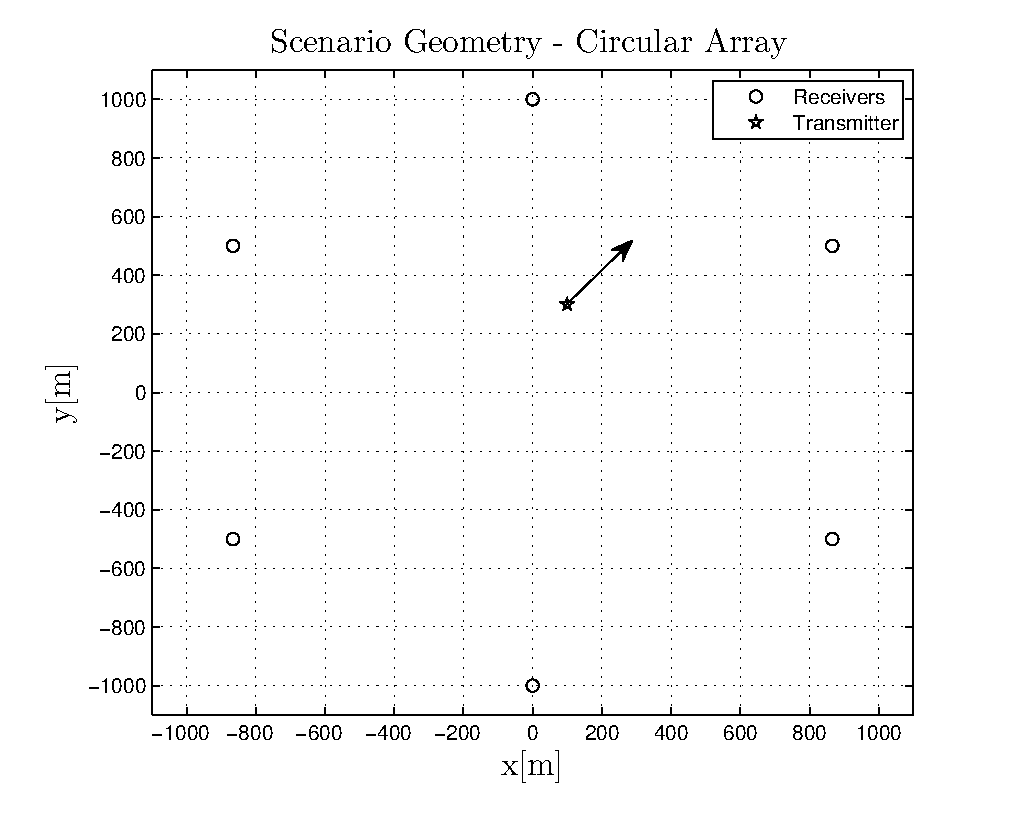
\includegraphics[scale=0.7]{scenario1.eps} 
\end{center}
\caption{Scenario Geometry: The 6 receivers are evenly spread on a circle with a radius of $1[km]$ around the origin. The transmitter is located at $(100,300)[m,m]$ with velocity $(200,200)[m/s,m/s]$.}
\label{fig:scenario1_geometry}
\end{figure}


\begin{figure}
\begin{center}
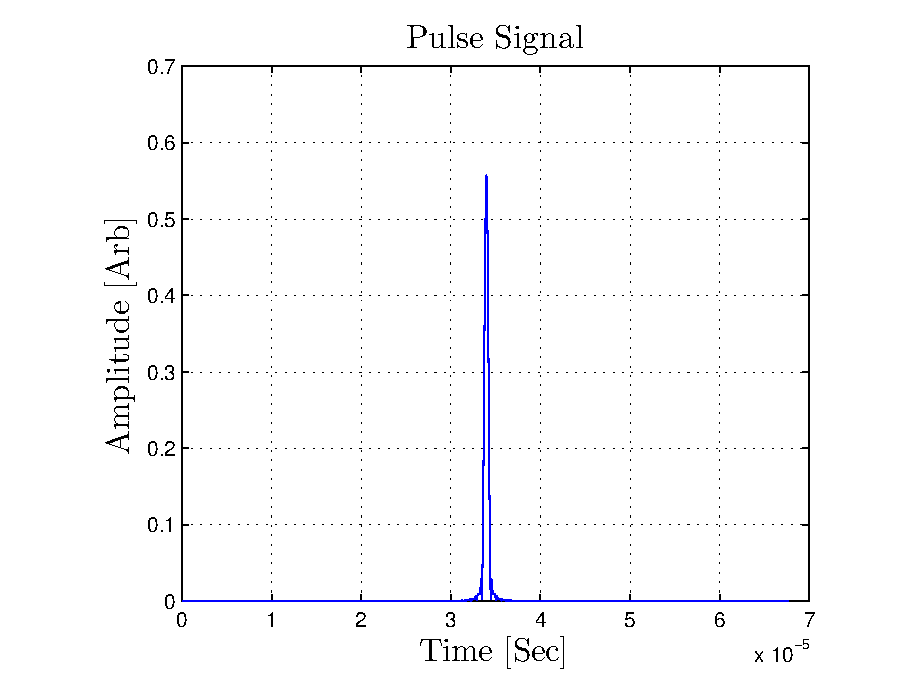
\includegraphics[scale=0.8]{pulseSignalAmp.eps} 
\end{center}
\caption{Time domain plot of the transmitted pulse signal}
\label{fig:pulseSignalAmp}
\end{figure}

\begin{figure}
\begin{center}
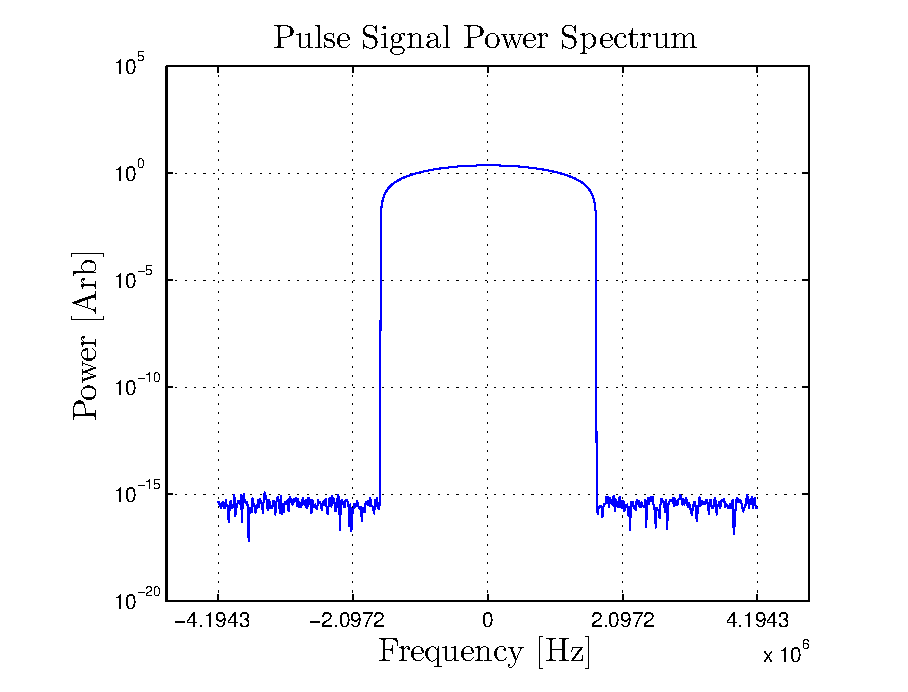
\includegraphics[scale=0.8]{pulseSignalFreq.eps} 
\end{center}
\caption{Power spectrum plot of the transmitted pulse signal}
\label{fig:pulseSignalFreq}
\end{figure}

\subsection*{Results}
As can be seen in figure (\ref{fig:scenario1_pos_rms}) and figure (\ref{fig:scenario1_vel_rms}) the direct one-step methods achieve better results than the conventional method.

Looking at figure (\ref{fig:scenario1_pos_rms}) we can see that in the examined SNRs, in the presented scenario, the known signals direct method achieves the position estimation CRLB for all of the examined SNR range.

Both the conventional two-step method and the direct unknown signals method achieve the bound at high SNR, but it is obvious that at lower SNR, the direct method shows better performance.

It is interesting to mention that both the known signals method, and the unknown signals methods achieve the known signals CRLB at high SNR. We would expect that only the known signals methods would achieve the known signals CRLB while the unknown signals methods would achieve the unknown signals CRLB, which is outside the scope of this work. Apparently, in this scenario, the unknown signals and the known signals CRLB are close enough so we are not able to distinct their asymptotic performance.

The superiority of the direct methods is less obvious in the results of the velocity estimation, as can be seen in figure (\ref{fig:scenario1_vel_rms}). Nevertheless, in spite of the noisy velocity estimations, it can be seen from figure (\ref{fig:scenario1_vel_rms}) that the direct methods show better performance than the conventional method, and that the known signals direct method shows better performance than the unknown signals method in lower SNRs.

It is interesting to notice that none of the velocity estimation methods reach the CRLB at any of the examined SNRs. A possible explanation is that the frequency shift caused by the Doppler effect in this scenario is extremely small compared to the sampling frequency divided by the number of samples, so that quantization errors in the simulation raise the effective noise level, and do not allow the performance achieve the CRLB.



\begin{figure}
\begin{center}
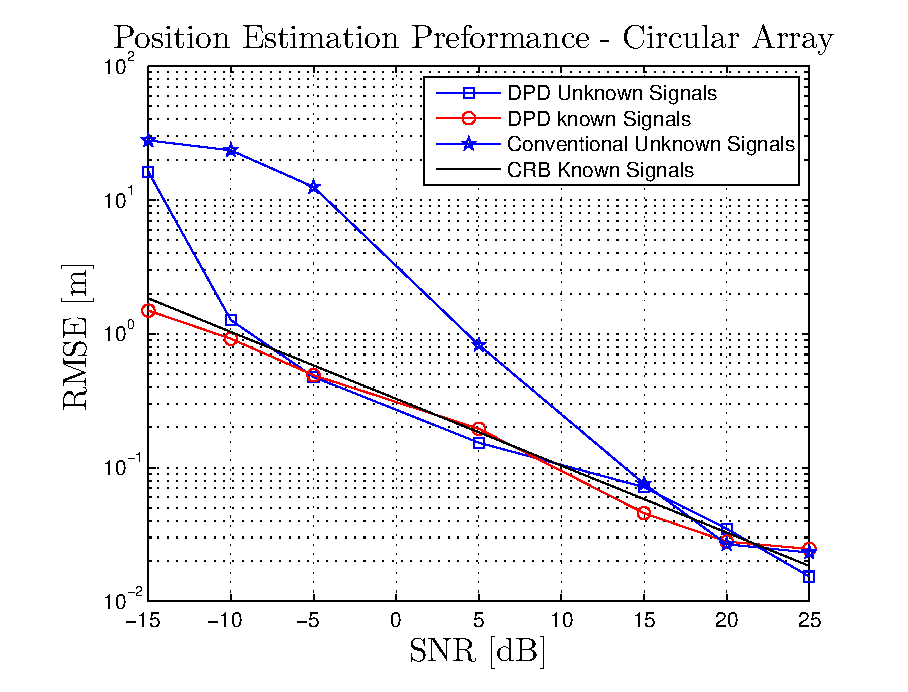
\includegraphics[scale=0.8]{scenario1pos.eps} 
\end{center}
\caption{Position Estimation Performance Vs. SNR - Circular Receivers Array}
\label{fig:scenario1_pos_rms}
\end{figure}

\begin{figure}
\begin{center}
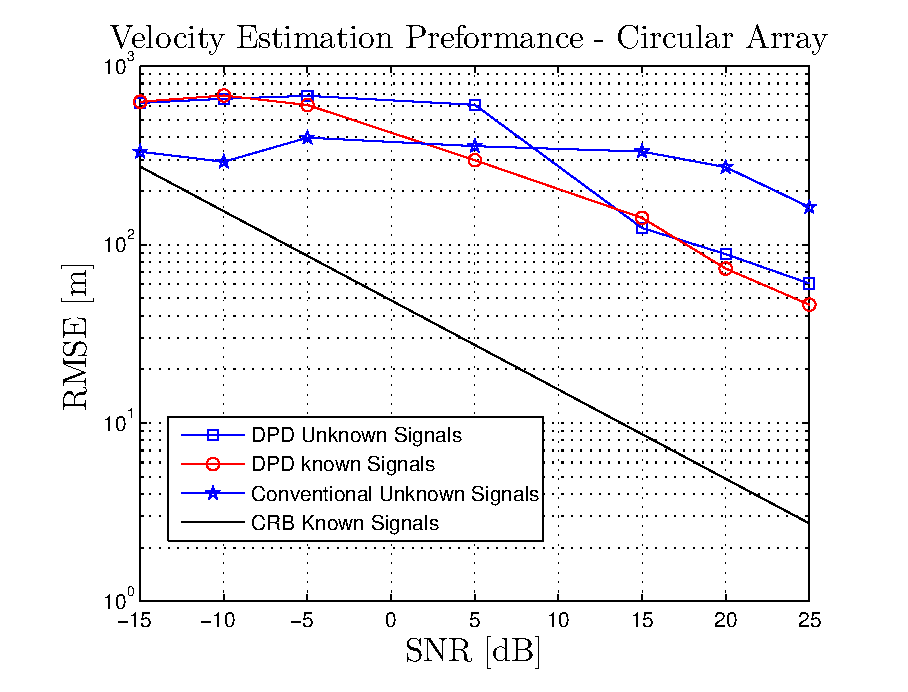
\includegraphics[scale=0.8]{scenario1vel.eps} 
\end{center}
\caption{Velocity Estimation Performance Vs. SNR - Circular Receivers Array}
\label{fig:scenario1_vel_rms}
\end{figure}

\section{Performance vs. SNR - Circular Receivers Array, Random Signal}

In this scenario, we used the same circular array geometry as in section (\ref{sec:performance_vs_snr_circular_pulse}), and the same transmitter position and velocity.

The transmitted signal is a random signal with a carrier frequency of $1$[GHz].
The signal is sampled with a sampling frequency of $2^{20}$[hz]$ \simeq 1$ [MHz].
The length of the sampling interval in each receiver is $512$ [samples]$ \simeq 488 $[$\mu$ Sec].\\
The simulated transmitted signal is a band-limited random signal.
Figure (\ref{fig:randSignalAmp}) shows random signal in the time domain. The power spectrum of the signal is shown in figure (\ref{fig:randSignalFreq}).

For every point on the graph, an average of $10$ estimations is taken.
Since the discussed problem requires the estimation of both the position and velocity of the transmitter, two parameters are calculated and presented in two different graphs for each SNR: The RMS of the positioning error, and the RMS of the velocity estimation error.

In this scenario, we compare the performance of the direct unknown signals method and the conventional two-step unknown signals method.

For the evaluation of the performance of the direct unknown signals method we use the $L3$ cost function.

For the evaluation of the performance of the conventional method, we use the two step method.
At the first step the TDOA and FDOA are estimated between each pair of receivers, and later used in a WLS cost function at the second step. We determine the optimal weights of the measurements using the known signals CRB for TOA and FOA measurements, as explained in subsection (\ref{subsec:tdoa_fdoa}).

The CRLB for known signals is presented on the graphs as well for reference.


\begin{figure}
\begin{center}
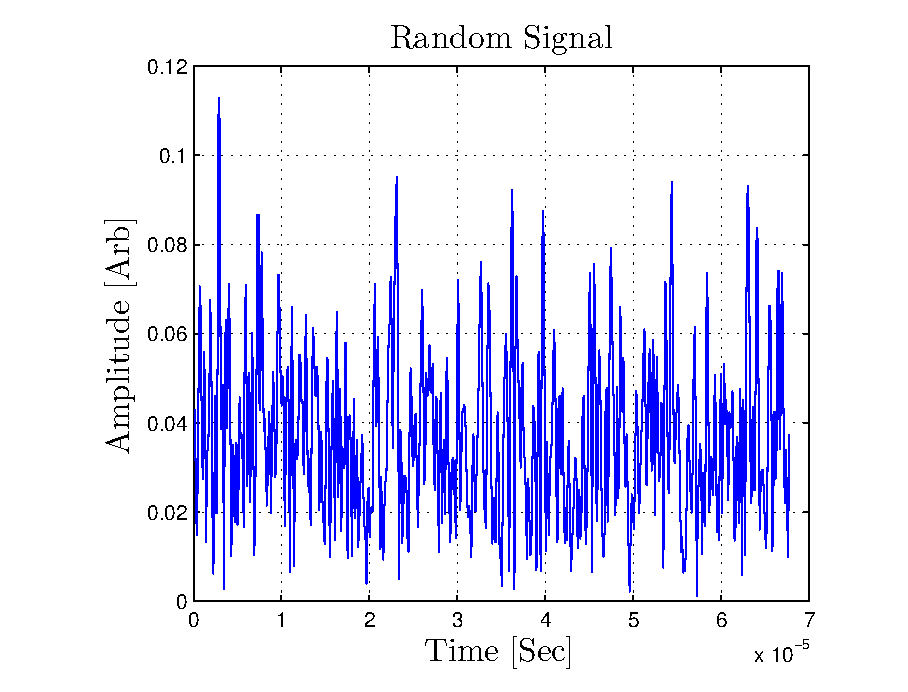
\includegraphics[scale=0.8]{randSignalAmp.eps} 
\end{center}
\caption{Time domain plot of the transmitted random signal}
\label{fig:randSignalAmp}
\end{figure}

\begin{figure}
\begin{center}
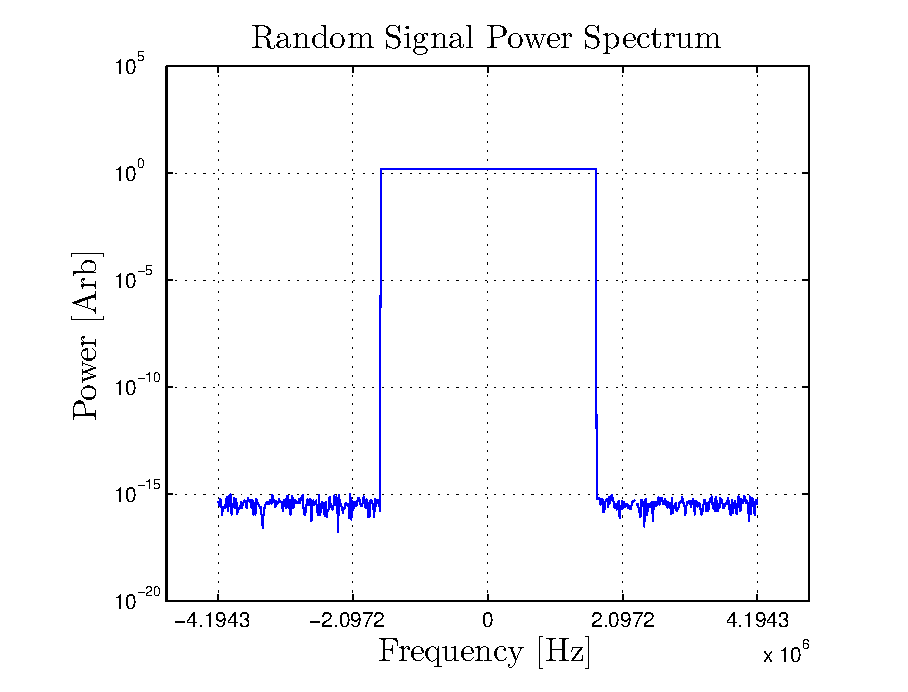
\includegraphics[scale=0.8]{randSignalFreq.eps} 
\end{center}
\caption{Power spectrum plot of the transmitted random signal}
\label{fig:randSignalFreq}
\end{figure}

\subsection*{Results}
As can be seen in figure (\ref{fig:scenario4_pos_rms}) and figure (\ref{fig:scenario4_vel_rms}) the direct one-step method achieves better results than the conventional two-step method.

Looking at figure (\ref{fig:scenario4_pos_rms}) we can see that in the examined SNRs, in the presented scenario, the known signals direct method achieves the position estimation CRLB for almost all of the examined SNR range.

Both the conventional two-step method and the direct unknown signals method achieve the bound at high SNR, but it is obvious that at lower SNR, the direct method shows better performance.

It is interesting to mention that both methods, which are both unknown signals methods, achieve the known signals CRLB at high SNR. We would expect that the unknown signals method would not achieve the known signals CRLB, whose derivation is outside the scope of this work. Apparently, in this scenario, the unknown signals and the known signals CRLB are close enough so we are not able to distinct between them.

The superiority of the suggested direct method is a little less obvious in the results of the velocity estimation, as can be seen in figure (\ref{fig:scenario4_vel_rms}). Nevertheless, in spite of the noisy velocity estimations, it can be seen from figure (\ref{fig:scenario4_vel_rms}) that both methods achieve the known-signals CRLB for almost all of the examined SNR range. Due to the noisy velocity estimations, it is hard to determine whether there is an advantage in the performance of the direct one-step method over the conventional two-step method.

Similarly to the position estimation performance, we note that although the two methods are unknown-signals methods, they achieve the known-signals CRLB for the velocity estimation performance as well. 

\begin{figure}
\begin{center}
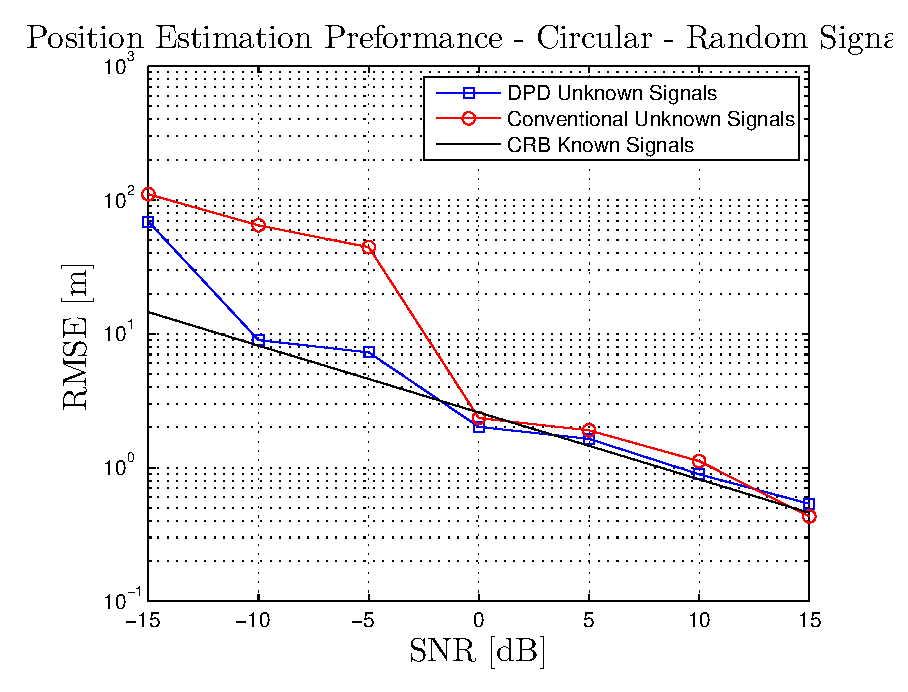
\includegraphics[scale=0.8]{scenario4pos.eps} 
\end{center}
\caption{Position Estimation Performance Vs. SNR - Circular Receivers Array, Random Signal}
\label{fig:scenario4_pos_rms}
\end{figure}

\begin{figure}
\begin{center}
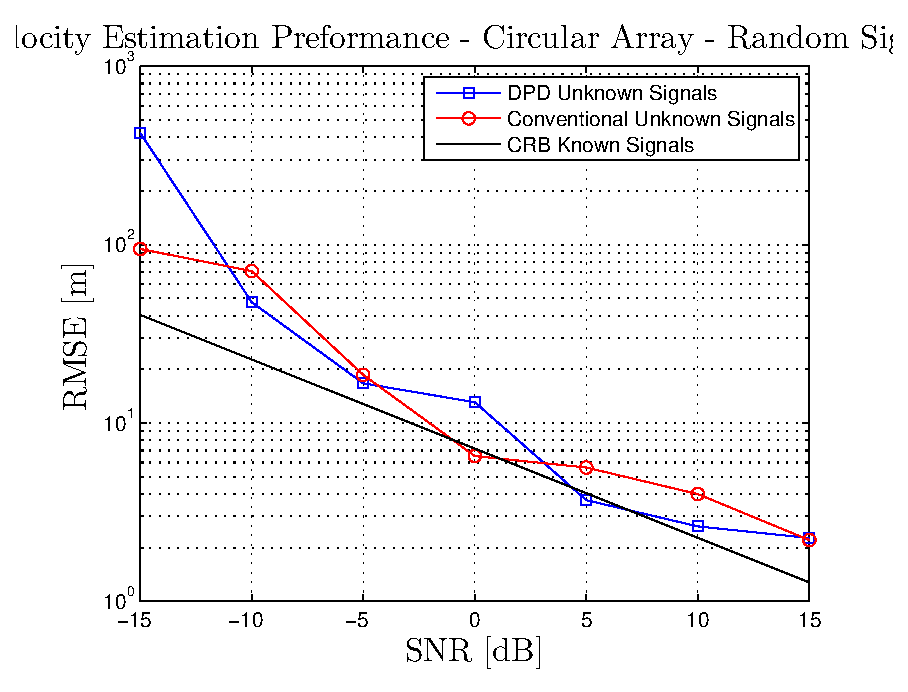
\includegraphics[scale=0.8]{scenario4vel.eps} 
\end{center}
\caption{Velocity Estimation Performance Vs. SNR - Circular Receivers Array, Random Signal}
\label{fig:scenario4_vel_rms}
\end{figure}


\section{Performance vs. SNR - Linear Receivers Array, Pulse Signal}

In this scenario, $6$ receivers are evenly spaced on the $x$-axis in a $2$[km] long linear array around the origin.
The transmitter is located $100$[m] away from the origin on the $x$-axis, and $1000$[m] away from the origin on the $y$-axis, as can be seen in figure (\ref{fig:scenario2_geometry}).
The transmitter's velocity is $200$[m/s] in the $x$ direction and $200$[m/s] in the $y$ direction.

The transmitted signal is a pulse signal with a carrier frequency of $1[GHz]$.
The signal is sampled with a sampling frequency of $2^{23}$[Hz]$ \simeq 8.4$ [MHz].
The length of the sampling interval in each receiver is $512$ [samples]$ \simeq 60 $[$\mu$ Sec].
The simulated transmitted signal is the same band-limited pulse signal that we used in section(\ref{sec:performance_vs_snr_circular_pulse}). Figure (\ref{fig:pulseSignalAmp}) shows the signal in the time-domain, while the power spectrum of the original transmitted signal is shown in figure (\ref{fig:pulseSignalFreq}).

For every point on the graph, an average of $10$ estimations is taken.
Since the discussed problem requires the estimation of both the position and the velocity of the transmitter, two parameters are calculated and presented in two different graphs for each SNR: The RMS of the positioning error, and the RMS of the velocity estimation error.

In this scenario, we compare the performance of the direct unknown signals method, the direct known signals method, and the conventional two-step method.
For known signals we use the $L2$ cost function in order to estimate the position and velocity of the transmitter. For unknown signals we use the $L3$ cost function.

For the evaluation of the performance of the conventional method, we use the two step method.
At the first step the TDOA and FDOA are estimated between each pair of receivers, and later used in a WLS cost function at the second step. We determine the optimal weights of the measurements using the known signals CRB for TOA and FOA measurements, as explained in subsection (\ref{subsec:tdoa_fdoa}).

The CRLB for known signals is presented on the graphs as well for reference.

\begin{figure}
\begin{center}
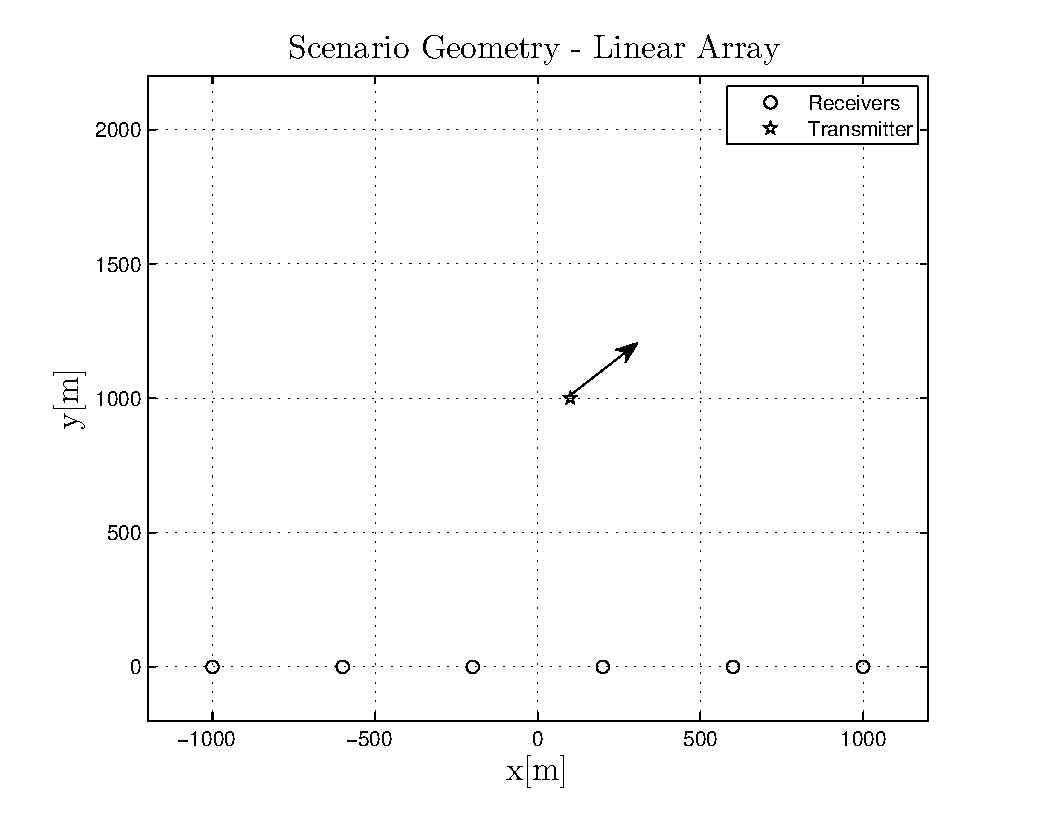
\includegraphics[scale=0.7]{scenario2.eps} 
\end{center}
\caption{Scenario Geometry: The 6 receivers are evenly spread on a the $x$-axis in a $2[km]$ long linear array around the origin. The transmitter is located at $(100,1000)$[m,m] with velocity $(200,200)$[m/s,m/s].}
\label{fig:scenario2_geometry}
\end{figure}


\subsection*{Results}
As can be seen in figure (\ref{fig:scenario2_pos_rms}) and figure (\ref{fig:scenario2_vel_rms}) the direct one-step methods achieve better results than the conventional two-step method.

In figure (\ref{fig:scenario2_pos_rms}) we can see that in the examined SNRs, in the presented scenario, the known signals direct one-step method achieves the position estimation CRLB for all of the examined SNR range.

Both the conventional two-step method and the direct unknown signals method do not achieve the known signals CRLB, but show a different kind of asymptotic behaviour. Because the derivation of the unknown signals CRLB is out of the scope of this work, we can only assume that both methods mentioned above achieve the unknown signals CRLB in high SNR. 

Nevertheless, although both methods show similar asymptotic behaviour in high SNR, it is clear that the direct unknown signals achieves better performance than the conventional method in low SNR scenarios.

The superiority of the suggested direct method is less obvious in the results of the velocity estimation, as can be seen in figure (\ref{fig:scenario2_vel_rms}). Nevertheless, in spite of the noisy velocity estimations, it can be seen from figure (\ref{fig:scenario2_vel_rms}) that the direct methods show better performance than the conventional method, and that the known signals direct method shows slightly better performance than the unknown signals method in lower SNRs.

It is interesting to notice that none of the velocity estimation methods achieve the CRLB at any of the examined SNRs. A possible explanation is that the frequency shift caused by the Doppler effect in this scenario is extremely small compared to the sampling frequency divided by the number of samples, so that quantization errors in the simulation raise the effective noise level, and do not allow the performance achieve the CRLB.

\begin{figure}
\begin{center}
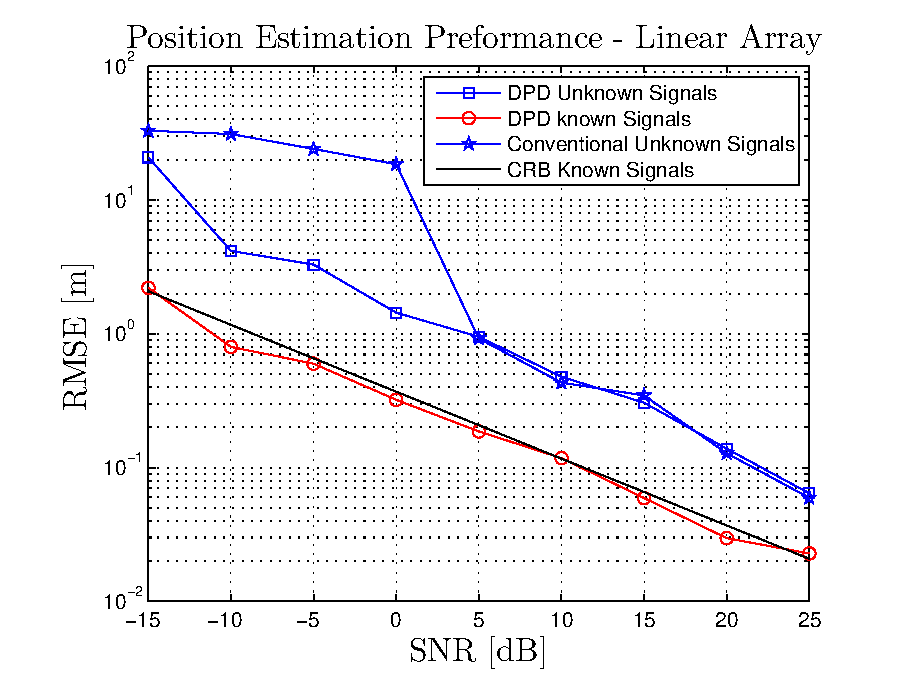
\includegraphics[scale=0.8]{scenario2pos.eps} 
\end{center}
\caption{Position Estimation Performance Vs. SNR - Linear Receivers Array, Pulse Signal}
\label{fig:scenario2_pos_rms}
\end{figure}

\begin{figure}
\begin{center}
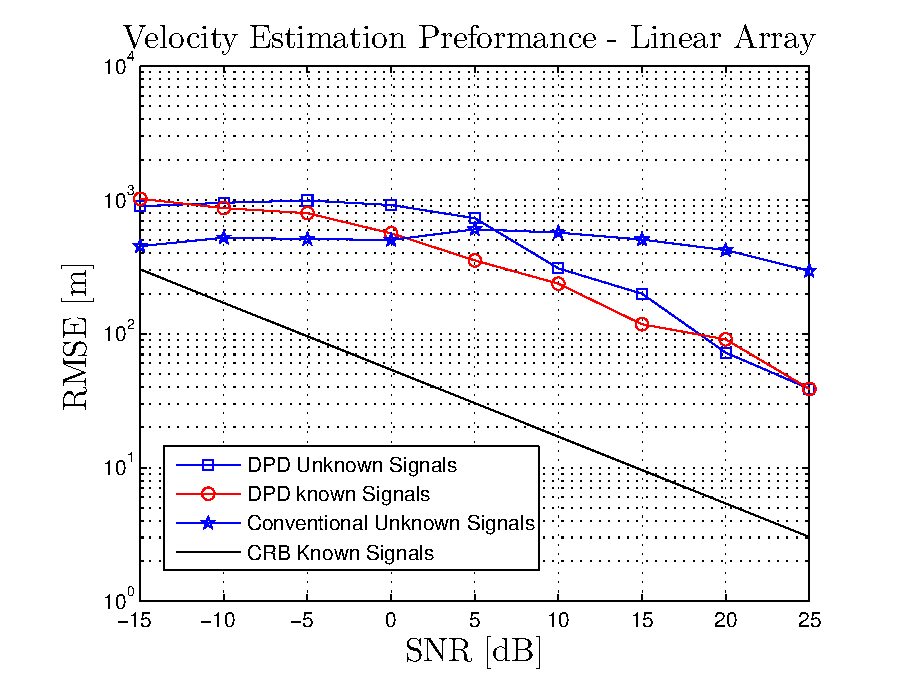
\includegraphics[scale=0.8]{scenario2vel.eps} 
\end{center}
\caption{Velocity Estimation Performance Vs. SNR - Linear Receivers Array, Pulse Signal}
\label{fig:scenario2_vel_rms}
\end{figure}

\section{Experimental Study Of The Cost Function}
\label{sec:experimental_study}
\subsection{General}
In the following section we present an experimental study, in which we show a few examples of the cost function. We present several contour plots to demonstrate the behaviour of the different cost functions, for several different geometries, and for different signal types.

We present the contour plots of the unknown signals, the known signals and the conventional cost functions, for pulse signals and for random signals, and for a linear array of receivers and for a circular array of receivers.

We present the different plots in order to provide a better understanding of the problem presented in this work and some intuition for it.

For creating the contour plots of the cost function we simulated a signal with a carrier frequency of $1$[GHz] sampled at a sampling frequency of $2^{23} \simeq 8.4$[MHz]. The sampled signals we used were $512$ samples long. The velocity of the transmitter was $(200,200)$ [m/s] in all of the simulated scenarios. Wherever a circular receivers array is mentioned, the circular array presented in figure (\ref{fig:scenario1_geometry}) is used, and whenever a linear receivers array is mentioned, the circular array presented in figure (\ref{fig:scenario2_geometry})

The cost functions presented were simulated in a noiseless environment with an infinite SNR, in order to demonstrate the behaviour of the cost function without the effect of noise.

The cost functions in this work are four-dimensional, they are evaluated in the two-dimensional position space and in the two-dimensional velocity space. Therefore, they are difficult to visualize. In this experimental study, we chose to demonstrate the behaviour of the cost functions in the two-dimensional position space, where the cost functions are evaluated at the true value of the velocity of the transmitter.


\subsection{Pulse Signals}

We start by examining the contour plots of the various cost functions for pulse signals. In this subsection, we use the same pulse signal described by figure (\ref{fig:pulseSignalAmp}) and figure (\ref{fig:pulseSignalFreq}), with the transmitter parameters described above.

\subsubsection*{Circular Array of Receivers}

Figure (\ref{fig:unknownSignalsPulseCircular}) presents the contour plot of the unknown signals one-step cost function for a circular array of receivers, figure (\ref{fig:knownSignalsPulseCircular}) presents the contour plot of the known signals one-step cost function and figure (\ref{fig:conventionalPulseCircular}) presents the contour plot of the conventional two-step cost function.

We notice that the one-step cost functions show mild apparent difference, as seen in figure (\ref{fig:unknownSignalsPulseCircular}) and (\ref{fig:knownSignalsPulseCircular}). 
We notice that for this scenario geometry, where the transmitter is located near the center of the circular array of receivers, the peak of the one-step cost functions is circular. 

We notice that the width of the peak around the transmitter is rather small. In order to find the peak for performing the position estimation, a high resolution grid is required. 

The cost function is clearly not convex outside of the area of the peak, so gradient based search methods can be used only for performing fine tuning once the peak was found, and cannot be used in order to find the peak.

We notice that there is some ambiguity in the cost function of the one-step methods, and some secondary peaks could be seen around the main peak. Although the value of the cost function at the real position of the transmitter is higher than its value at the secondary peaks, these peaks might prevent the algorithm from finding the real position of the transmitter, if the resolution of the grid search is not high enough.

As can be seen in figure (\ref{fig:conventionalPulseCircular}), the peak around the real position of the transmitter is rather wide, there are no apparent ambiguities, and the cost-function is convex for a wide area. 
As can be seen further in a wider view of the conventional cost function in figure (\ref{fig:zoomoutConventionalPulseCircular}), the cost-function maintains its convexity for a much wider area than the one-step methods.
Thus, using gradient based methods, and avoiding grid search is possible with the conventional cost function.

\begin{figure}
\begin{center}
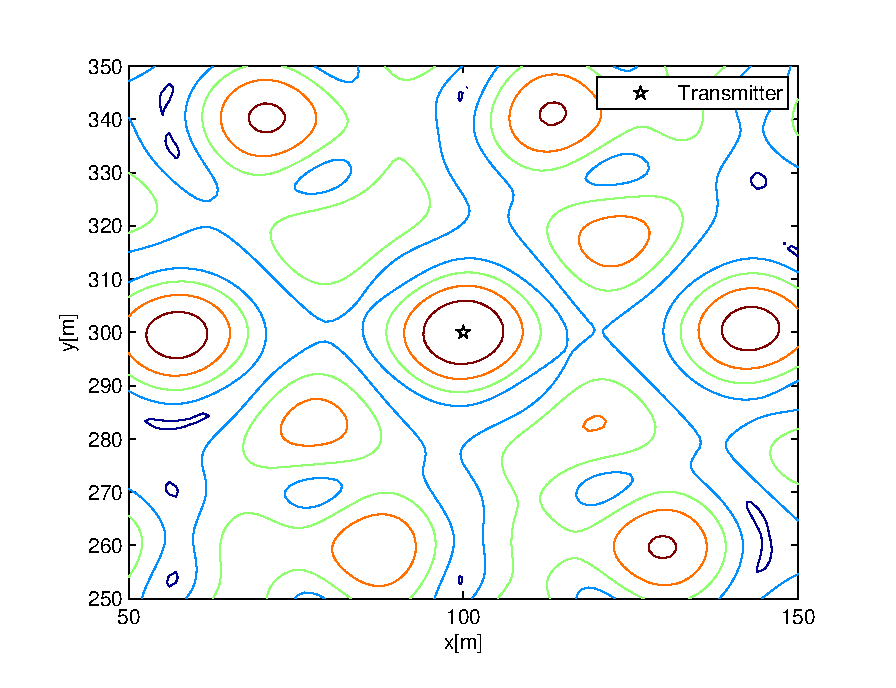
\includegraphics[scale=0.8]{plots-1-unknownSignalsPulseCircular.eps} 
\end{center}
\caption{Contour plot of the unknown signals cost function, for a circular receivers array and a pulse signal}
\label{fig:unknownSignalsPulseCircular}
\end{figure}

\begin{figure}
\begin{center}
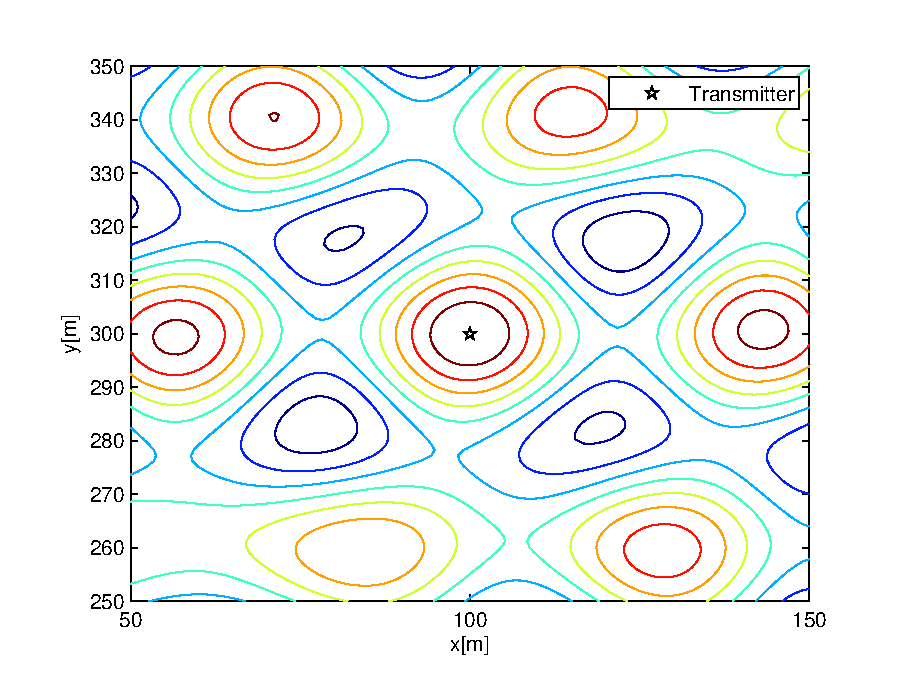
\includegraphics[scale=0.8]{plots-2-knownSignalsPulseCircular.eps} 
\end{center}
\caption{Contour plot of the known signals cost function, for a circular receivers array and a pulse signal}
\label{fig:knownSignalsPulseCircular}
\end{figure}

\begin{figure}
\begin{center}
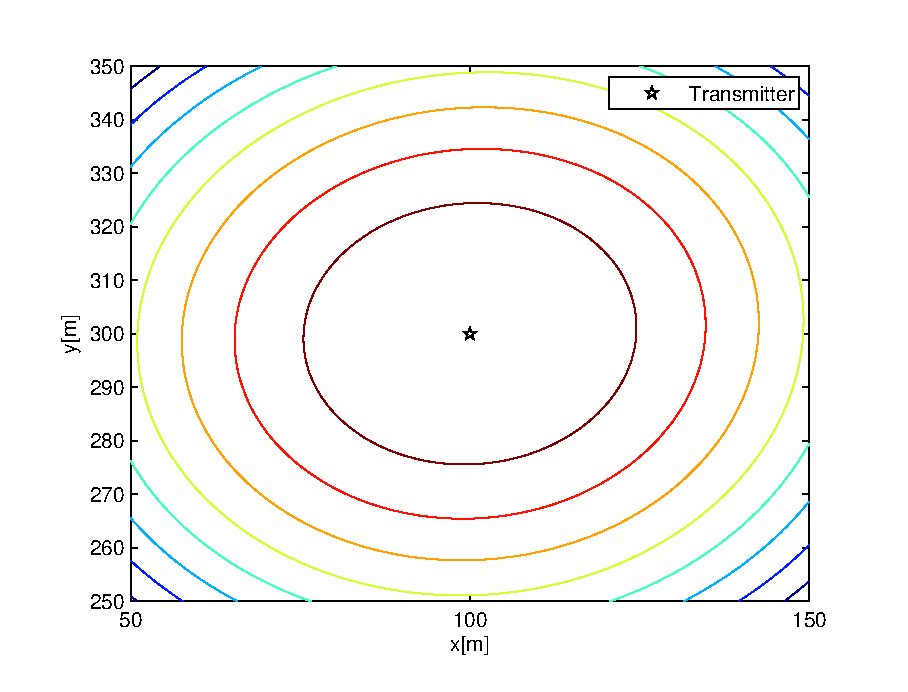
\includegraphics[scale=0.8]{plots-3-ConventionalPulseCircular.eps} 
\end{center}
\caption{Contour plot of the conventional two-step cost function, for a circular receivers array and a pulse signal}
\label{fig:conventionalPulseCircular}
\end{figure}

\begin{figure}
\begin{center}
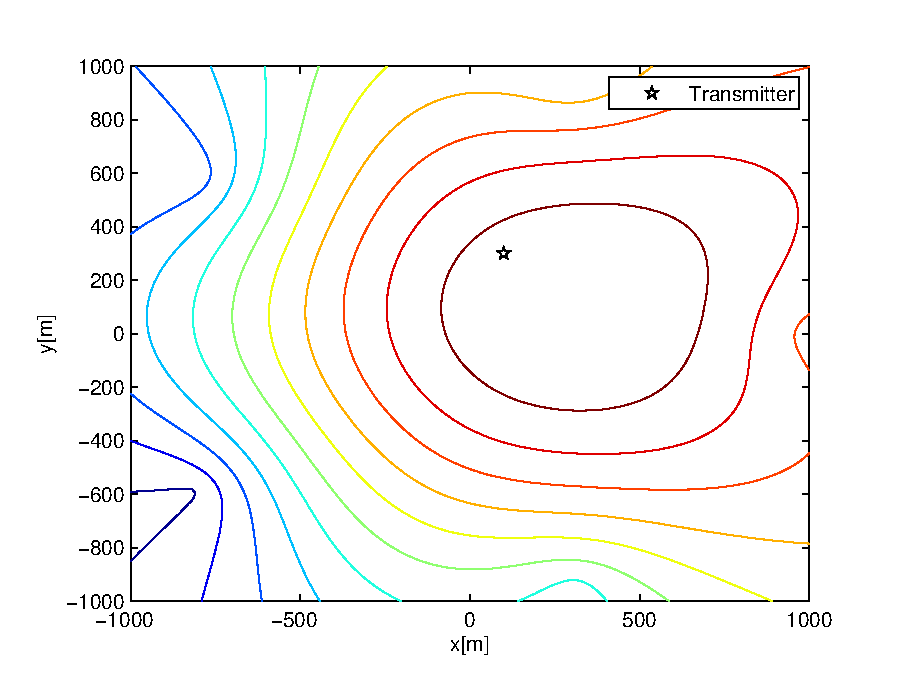
\includegraphics[scale=0.8]{plots-4-ConventionalPulseCircularZoomOut.eps} 
\end{center}
\caption{Wide view contour plot of the conventional two-step cost function, for a circular receivers array and a pulse signal}
\label{fig:zoomoutConventionalPulseCircular}
\end{figure}

\subsubsection*{Linear Array of Receivers}
Figure (\ref{fig:unknownSignalsPulseLinear}) presents the contour plot of the unknown signals one-step cost function for a linear array of receivers, figure (\ref{fig:knownSignalsPulseLinear}) presents the contour plot of the known signals one-step cost function and figure (\ref{fig:conventionalPulseLinear}) presents the contour plot of the conventional two-step cost function.

We notice that contrary to the previous scenario, in this scenario there is a significant difference between all of the cost functions.

In figure (\ref{fig:unknownSignalsPulseLinear}) we can see that in this scenario the peak of the cost function around the position of the transmitter is no longer circular, but rather elliptical.

The known signals cost function, on the other hand, keeps the same peak characteristics as in the circular array of receivers scenario, as can be seen in figure (\ref{fig:knownSignalsPulseLinear}).

We notice that in the cost function of both one-step methods, the width of the peak around the transmitter is rather small. In order to find the peak for performing the position estimation, a high resolution grid is required. 

The cost function of both one-step methods is clearly not convex outside of the area of the peak, so gradient based search methods can be used only for performing fine tuning once the peak was found, and cannot be used in order to find the peak.

We notice that there is some ambiguity in the cost function of the one-step methods, and some secondary peaks could be seen around the main peak. Although the value of the cost function at the real position of the transmitter is higher than its value at the secondary peaks, these peaks might prevent the algorithm from finding the real position of the transmitter, if the resolution of the grid search is not high enough.

As can be seen in figure (\ref{fig:conventionalPulseLinear}), the peak around the real position of the transmitter is rather wide, there are no apparent ambiguities, and the cost-function is convex for a wide area. 
As can be seen further in a wider view of the conventional cost function in figure (\ref{fig:zoomoutConventionalPulseLinear}), the cost-function maintains its convexity for a much wider area than the one-step methods.
Thus, using gradient based methods, and avoiding grid search is possible with the conventional cost function.

\begin{figure}
\begin{center}
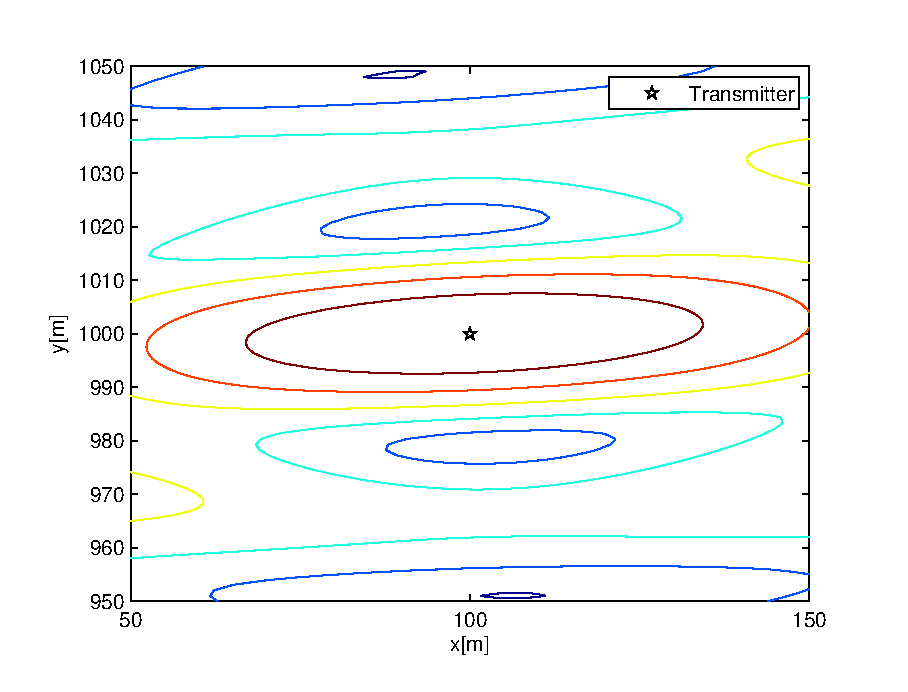
\includegraphics[scale=0.8]{plots-5-unknownSignalsPulseLinear.eps} 
\end{center}
\caption{Contour plot of the unknown signals cost function, for a linear receivers array and a pulse signal}
\label{fig:unknownSignalsPulseLinear}
\end{figure}

\begin{figure}
\begin{center}
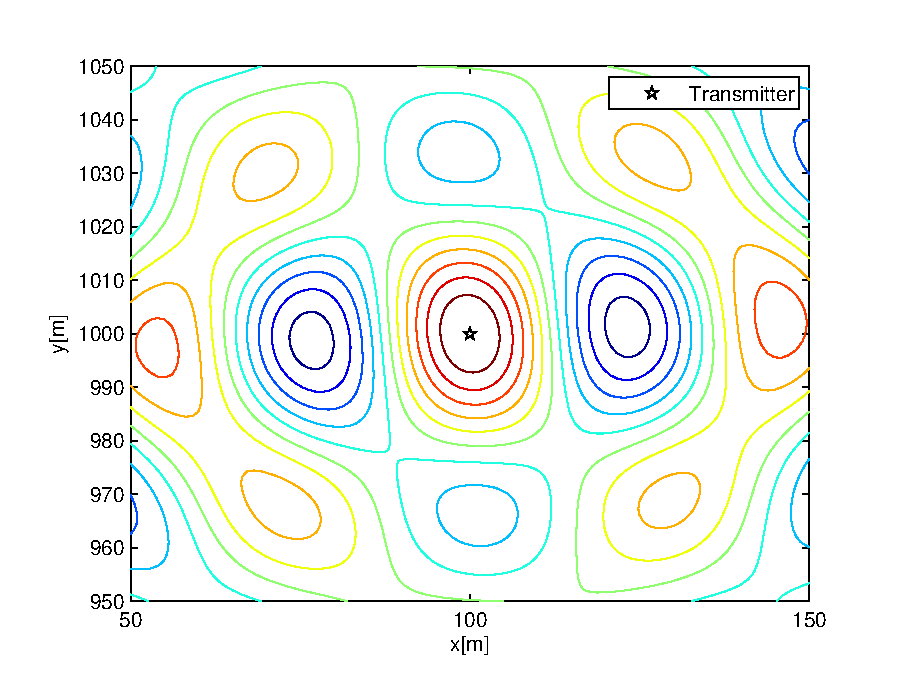
\includegraphics[scale=0.8]{plots-6-knownSignalsPulseLinear.eps} 
\end{center}
\caption{Contour plot of the known signals cost function, for a linear receivers array and a pulse signal}
\label{fig:knownSignalsPulseLinear}
\end{figure}

\begin{figure}
\begin{center}
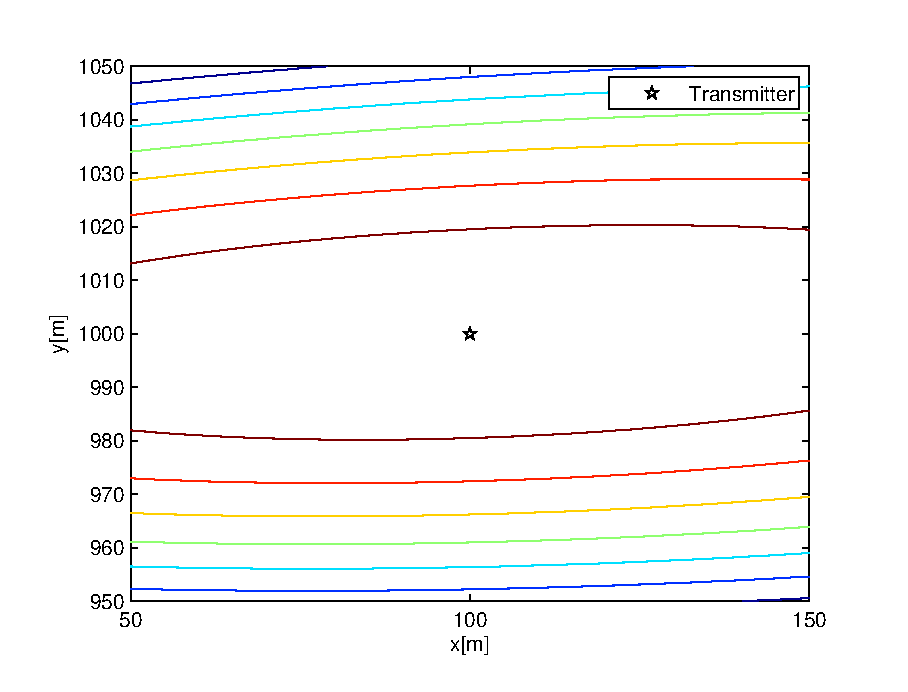
\includegraphics[scale=0.8]{plots-7-ConventionalPulseLinear.eps} 
\end{center}
\caption{Contour plot of the conventional two-step cost function, for a linear receivers array and a pulse signal}
\label{fig:conventionalPulseLinear}
\end{figure}

\begin{figure}
\begin{center}
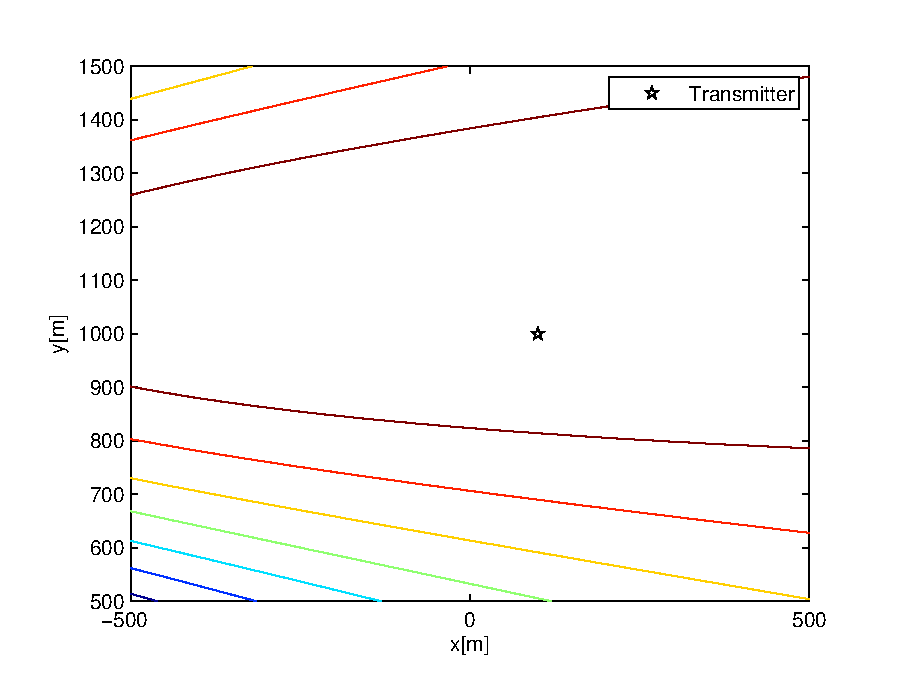
\includegraphics[scale=0.8]{plots-8-ConventionalPulseLinearZoomOut.eps} 
\end{center}
\caption{Wide view contour plot of the conventional two-step cost function, for a linear receivers array and a pulse signal}
\label{fig:zoomoutConventionalPulseLinear}
\end{figure}

\subsection{Random Signals}
We continue by examining the contour plots of the various cost functions for random signals. Since the properties of the cost function strongly depend on the properties of the signal, it is interesting to examine the cost function of different signals.
In this subsection, we use the same random signal described by figure (\ref{fig:randSignalAmp}) and figure (\ref{fig:randSignalFreq}), with the transmitter parameters described above.

\subsubsection*{Circular Array of Receivers}
Figure (\ref{fig:unknownSignalsRandCircular}) presents the contour plot of the unknown signals one-step cost function for a circular array of receivers, figure (\ref{fig:knownSignalsRandCircular}) presents the contour plot of the known signals one-step cost function and figure (\ref{fig:conventionalRandCircular}) presents the contour plot of the conventional two-step cost function.

We notice that the one-step unknown signals cost function for the random signal has a smaller peak than for the pulse signal, and less ambiguity, as is demonstrated further by figure (\ref{fig:unknownSignalRandCircularZoomout}).

For the one-step known signals cost function we see that there is a slightly larger peak than the unknown-signals cost function. Some significant ambiguity is also apparent, as can be further seen in figure (\ref{fig:knownSignalRandCircularZoomout}).

We notice that for this scenario geometry, where the transmitter is located near the center of the circular array of receivers, the peak of the one-step cost functions is circular. 

We notice that the width of the peak around the transmitter is rather small. In order to find the peak for performing the position estimation, a high resolution grid is required. 

The cost function is clearly not convex outside of the area of the peak, so gradient based search methods can be used only for performing fine tuning once the peak was found, and cannot be used in order to find the peak.

As can be seen in figure (\ref{fig:conventionalRandCircular}), the peak of the conventional two-step cost function around the real position of the transmitter is rather wide, there are no apparent ambiguities, and the cost-function is convex for a wide area. 

As can be seen further in a wider view of the conventional cost function in figure (\ref{fig:conventionalSignalRandCircularZoomout}), the cost-function maintains its convexity for a much wider area than the one-step methods.
Thus, using gradient based methods, and avoiding grid search is possible with the conventional cost function.

\begin{figure}
\begin{center}
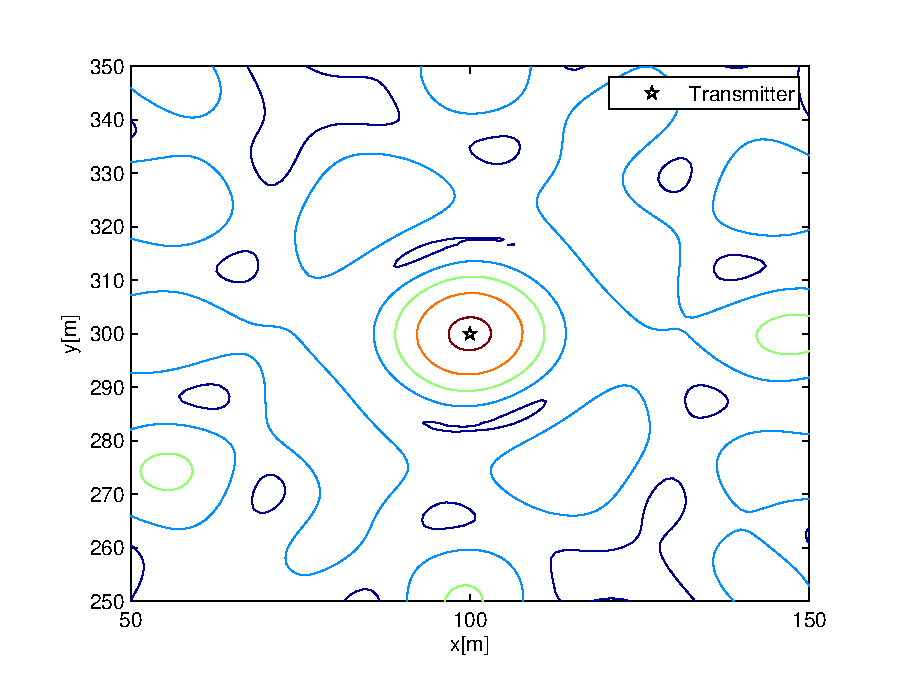
\includegraphics[scale=0.8]{plots-9-unknownSignalsRandCircular.eps} 
\end{center}
\caption{Contour plot of the unknown signals cost function, for a circular receivers array and a random signal}
\label{fig:unknownSignalsRandCircular}
\end{figure}

\begin{figure}
\begin{center}
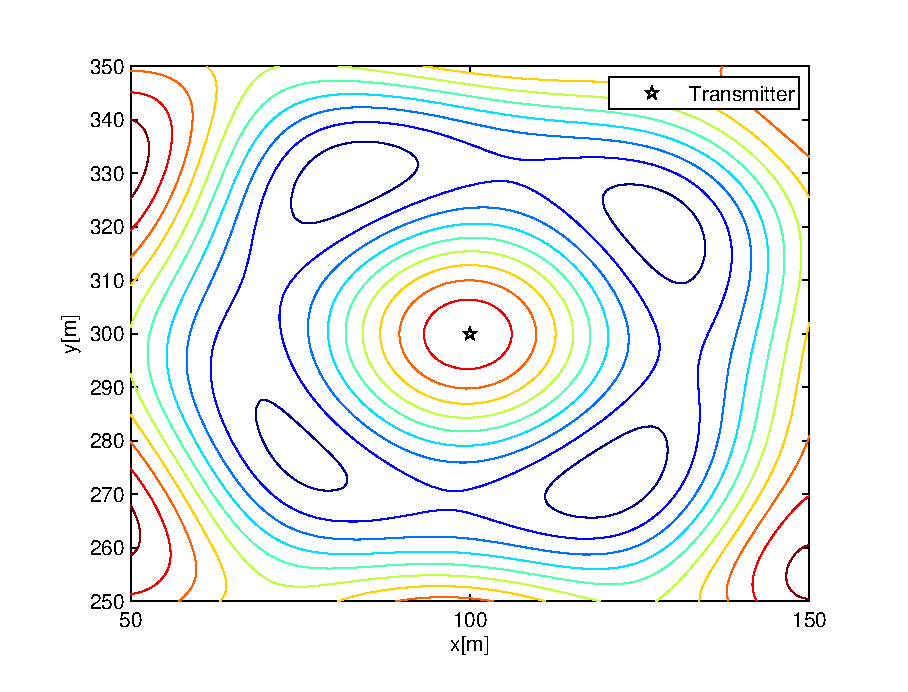
\includegraphics[scale=0.8]{plots-10-knownSignalsRandCircular.eps} 
\end{center}
\caption{Contour plot of the known signals cost function, for a circular receivers array and a random signal}
\label{fig:knownSignalsRandCircular}
\end{figure}

\begin{figure}
\begin{center}
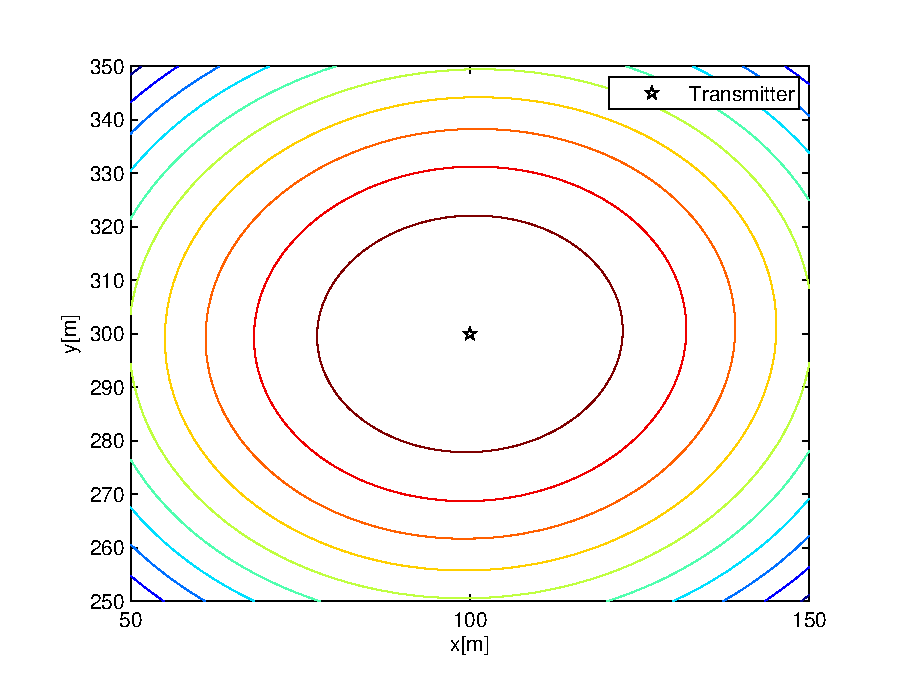
\includegraphics[scale=0.8]{plots-11-ConventionalRandCircular.eps} 
\end{center}
\caption{Contour plot of the conventional two-step signals cost function, for a circular receivers array and a random signal}
\label{fig:conventionalRandCircular}
\end{figure}

\begin{figure}
\begin{center}
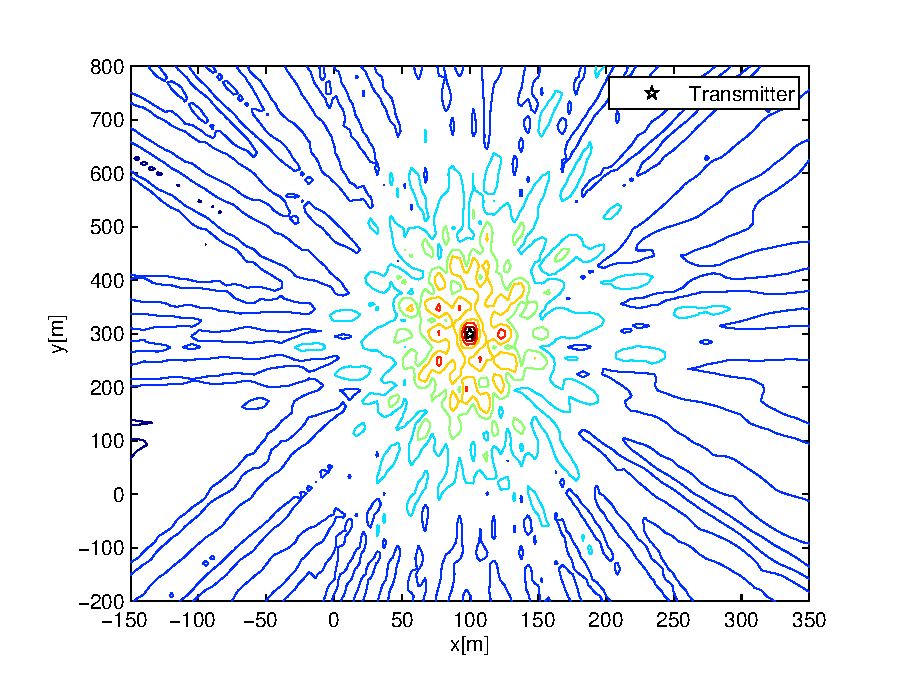
\includegraphics[scale=0.8]{plots-17-unknownSignalRandCircularZoomout.eps} 
\end{center}
\caption{Wide view contour plot of the unknown signals cost function, for a circular receivers array and a random signal}
\label{fig:unknownSignalRandCircularZoomout}
\end{figure}

\begin{figure}
\begin{center}
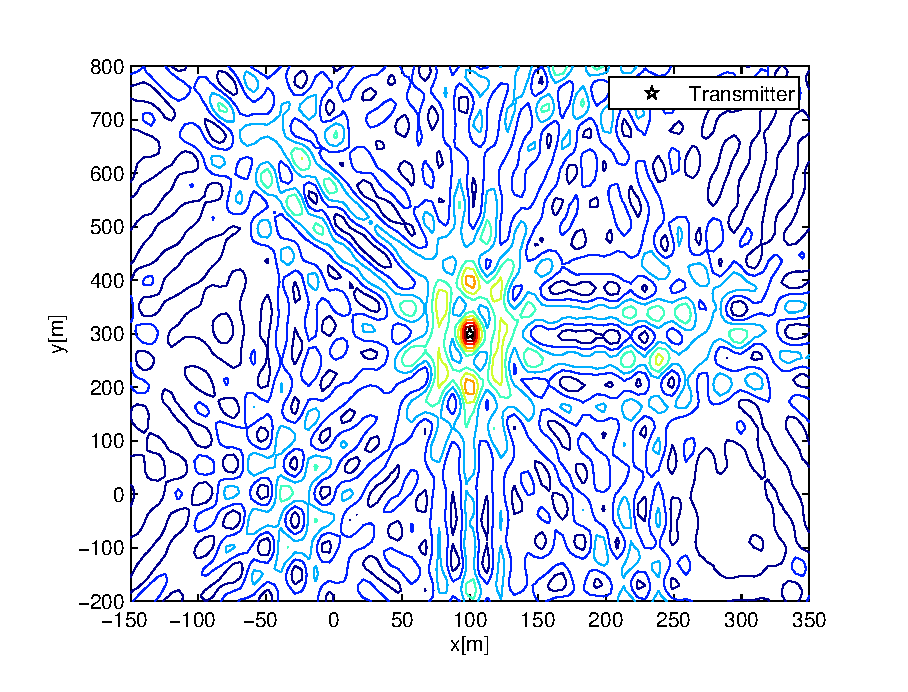
\includegraphics[scale=0.8]{plots-18-knownSignalRandCircularZoomout.eps} 
\end{center}
\caption{Wide view contour plot of the known signals cost function, for a circular receivers array and a random signal}
\label{fig:knownSignalRandCircularZoomout}
\end{figure}

\begin{figure}
\begin{center}
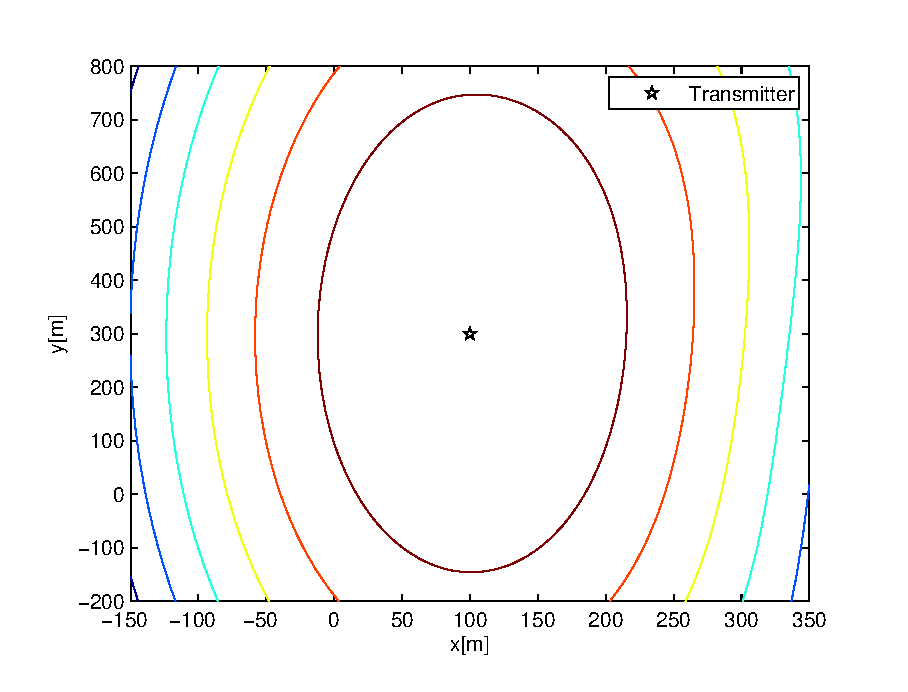
\includegraphics[scale=0.8]{plots-19-ConventionalRandCircularZoomout.eps} 
\end{center}
\caption{Wide view contour plot of the conventional two-step cost function, for a circular receivers array and a random signal}
\label{fig:conventionalSignalRandCircularZoomout}
\end{figure}

\subsubsection*{Linear Array of Receivers}
Figure (\ref{fig:unknownSignalsRandLinear}) presents the contour plot of the unknown signals one-step cost function for a circular array of receivers, figure (\ref{fig:knownSignalsRandLinear}) presents the contour plot of the known signals one-step cost function and figure (\ref{fig:conventionalRandLinear}) presents the contour plot of the conventional two-step cost function.

We notice that the one-step unknown signals cost function for the random signal has slightly less ambiguity than for the pulse signal, as is demonstrated further by figure (\ref{fig:unknownSignalRandLinearZoomout}).
As in the case of the pulse signal, we see that the peak of the one-step unknown signals method has an elliptical shape.

The one-step known signals cost function for the random signal shows great similarity to the known signals cost function for the pulse signal. Significant ambiguity around the main peak is demonstrated by figure (\ref{fig:unknownSignalRandLinearZoomout}).

We notice that the width of the peak of the one-step methods around the transmitter is rather small. In order to find the peak for performing the position estimation, a high resolution grid is required. 

The cost function is clearly not convex outside of the area of the peak, so gradient based search methods can be used only for performing fine tuning once the peak was found, and cannot be used in order to find the peak.

As can be seen in figure (\ref{fig:conventionalRandLinear}), the peak of the conventional two-step cost function around the real position of the transmitter is rather wide, there are no apparent ambiguities, and the cost-function is convex for a wide area. 

\begin{figure}
\begin{center}
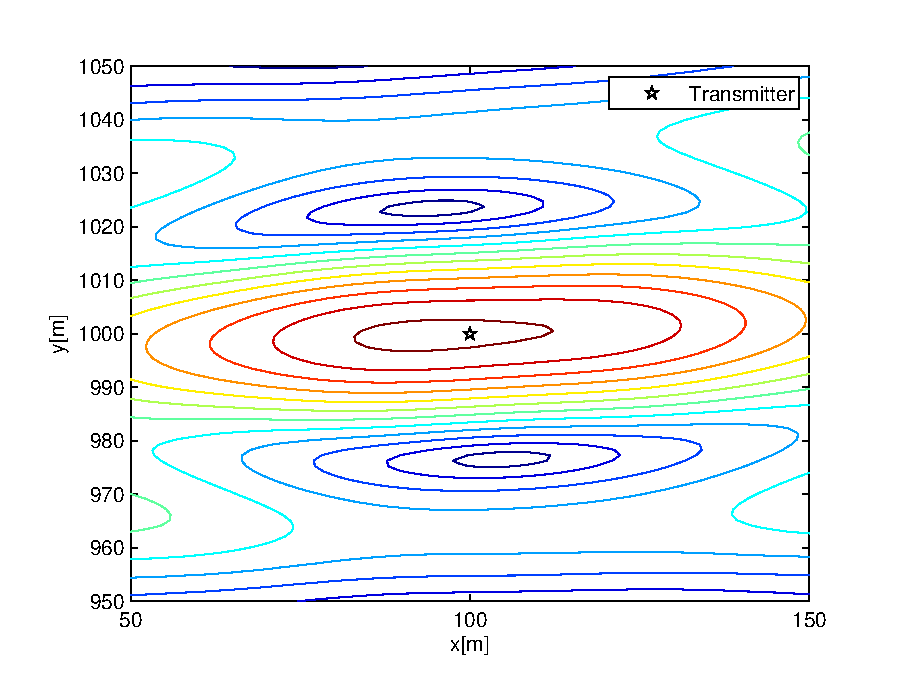
\includegraphics[scale=0.8]{plots-12-UnknownSignalRandLinear.eps} 
\end{center}
\caption{Contour plot of the unknown signals cost function, for a linear receivers array and a random signal}
\label{fig:unknownSignalsRandLinear}
\end{figure}

\begin{figure}
\begin{center}
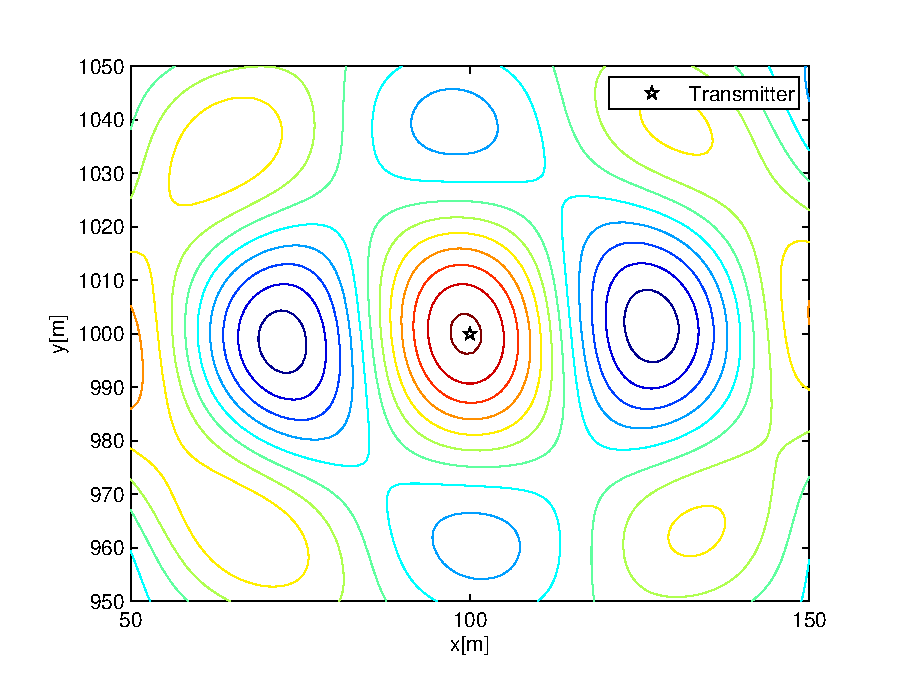
\includegraphics[scale=0.8]{plots-13-knownSignalRandLinear.eps} 
\end{center}
\caption{Contour plot of the known signals cost function, for a linear receivers array and a random signal}
\label{fig:knownSignalsRandLinear}
\end{figure}

\begin{figure}
\begin{center}
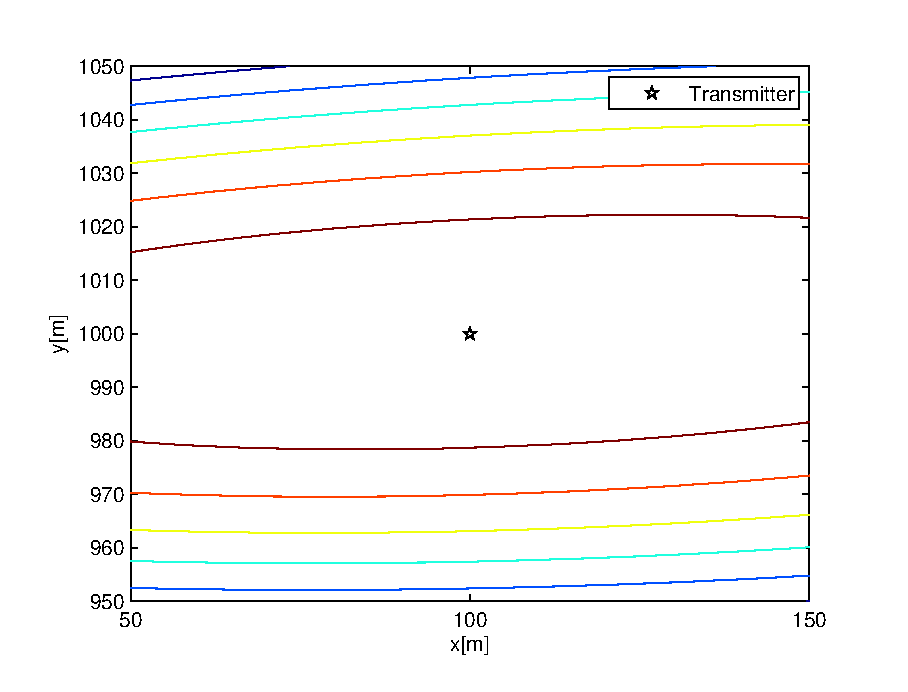
\includegraphics[scale=0.8]{plots-14-ConventionalRandLinear.eps} 
\end{center}
\caption{Contour plot of the conventional two-step signals cost function, for a linear receivers array and a random signal}
\label{fig:conventionalRandLinear}
\end{figure}

\begin{figure}
\begin{center}
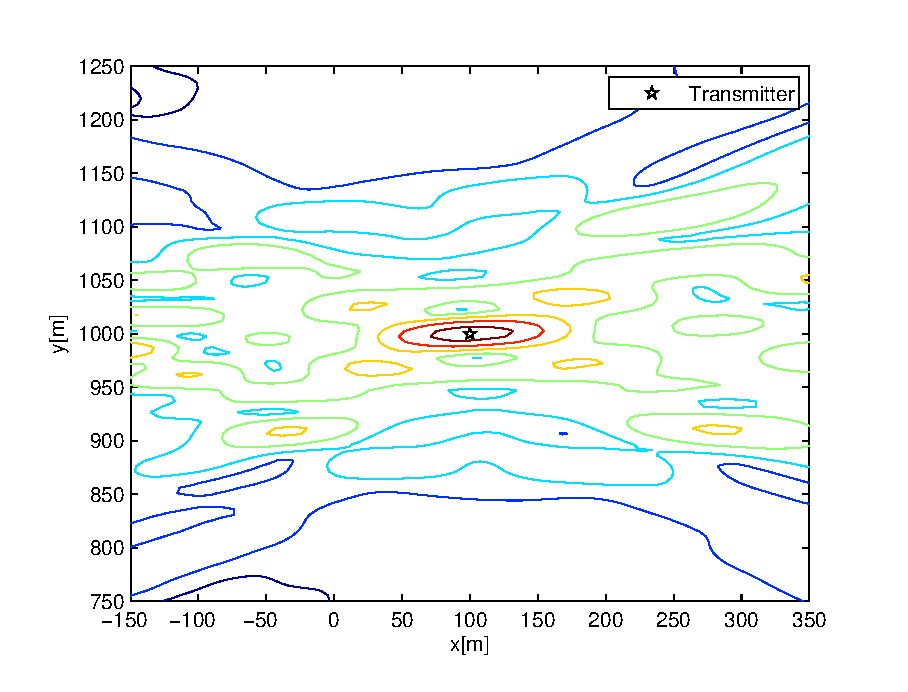
\includegraphics[scale=0.8]{plots-15-UnknownSignalRandLinearZoomout.eps} 
\end{center}
\caption{Wide view contour plot of the unknown signals cost function, for a linear receivers array and a random signal}
\label{fig:unknownSignalRandLinearZoomout}
\end{figure}

\begin{figure}
\begin{center}
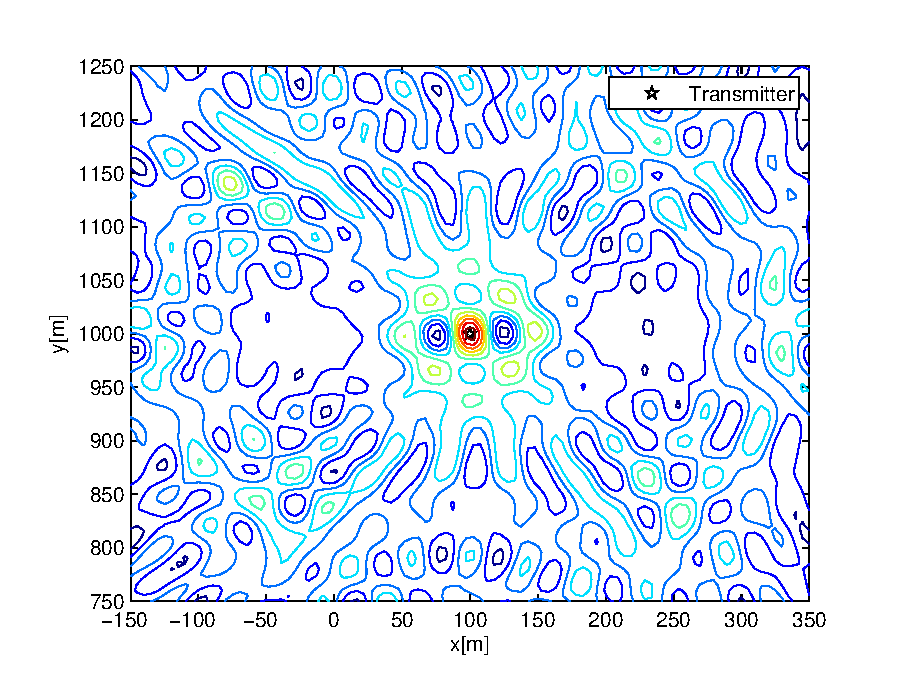
\includegraphics[scale=0.8]{plots-16-knownSignalRandLinearZoomout.eps} 
\end{center}
\caption{Wide view contour plot of the known signals cost function, for a linear receivers array and a random signal}
\label{fig:knownSignalRandLinearZoomout}
\end{figure}


\section{Performance Vs. Transmitter Position}

In this section we explore the relation between the performance of the algorithm, and the scenario geometry. 
We explore the expected performance of the algorithm for different positions of the transmitter in relation to the receivers array. We present the results of this simulation for a circular array of receivers and for a linear array of receivers. Nevertheless, this method could be applied to any arbitrary array of receivers, and could be used in order to design optimal receivers geometry for a given scenario.

Designing an optimal receivers array strongly depends on the characteristics of the problem, on its constraints and on the definition of the goals of the system \cite{fowler_wu}. Possible constraints could be the number of available receivers and the area on which they can lye. Possible definitions of the goals of the system could be maximizing the performance for a single possible transmitter position, or maximizing the average performance over an area on which the transmitter lies. Since the problem of designing an optimal receivers array depends on describing a specific scenario, we will only describe a method that enables customizing the design for a specific scenario.

In order to estimate the performance of the algorithm in this section, we only used the results of the CRB, 
and did not use true simulation results of our suggested algorithm. The main reason for doing that is that in order to create a good quality contour plot of the expected performance, the performance has to be evaluated in many different positions. Performing Monte-Carlo simulations shows much better computational complexity than calculating the CRB at a given position, and as we know from theory and as we presented in the previous simulations, the performance of our estimator is asymptotically efficient, so that calculating the CRB gives us a good estimate of the performance of our algorithm.

For each receiver array geometry we created a two contour plots, one for the position estimation performance, and one for the velocity estimation performance. The height of every point on the plot represents the calculated CRB for a transmitter with the above parameters, transmitting from that point. In order to make the plots more informative, we present the calculated CRB on a logarithmic scale, where the height of every point is the $\text{log}_{10}$ of the CRB at that point. The contour lines are equally on a logarithmic scale.

The parameters used for the simulation in this section are similar to the parameters used in the above sections. For this simulation, we used $512$ samples of a random signal, transmitted with a carrier frequency of $1$[GHz], and sampled with a $2^{15} \simeq 32$[KHz] sampling frequency with a $25$[dB] SNR in all of the receivers. The velocity of the transmitter in all of the simulations in this section is $[200,200]$[m/s].

\subsubsection*{Circular Receivers Array}
For analysing the circular receivers array scenario, we used the receivers array described in figure (\ref{fig:scenario1_geometry}), where there are 6 receivers arranged on a circle with a radius of $1$[km].

From figures (\ref{fig:CRBRandCircularPosition}) and (\ref{fig:CRBRandCircularVelocity}) we can learn that for this scenario, the spatial behaviour of the estimation performance of the position and of the estimation performance of the velocity is quite similar.

From both figures, we can learn that the best estimation performance of a circular array is inside the circle. We can see that the estimation performance is almost uniform inside the circle, where there is slightly better performance near the center of the circle.

Outside the circle, we can see that the performance decreases the farther the transmitter is from the center of the circle. 

Here, an interesting phenomenon can be noticed. While the position estimation performance is more or less isotropic, the velocity estimation performance declines dramatically when the moving away from the center of the circle in the direction of the speed of the transmitter. We can explain the decline in performance on that line, in the fact that on the line that goes through the center of the circle in the direction of the velocity of the transmitter, the differential Doppler effect is minimal, and the difference between the received frequency in the receivers is minimal. Thus, the estimation of the velocity, whose information is found only in the frequency difference is affected. 

This phenomenon can be observed also in the position estimation performance, but it is less dominant, since the information about the position of the transmitter is found both in the time difference, and in the frequency difference of the received signals.


\begin{figure}
\begin{center}
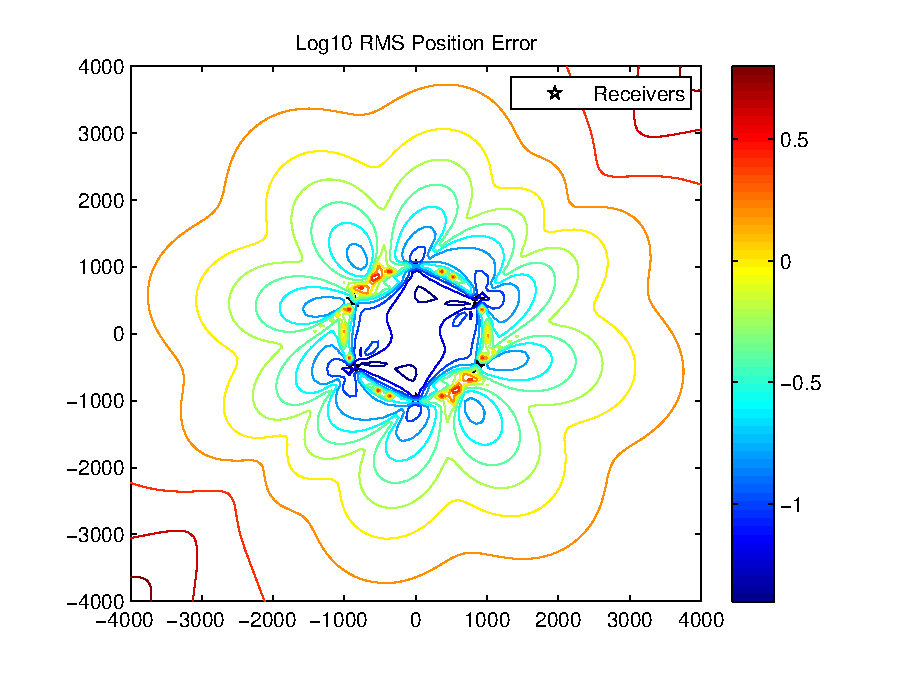
\includegraphics[scale=0.8]{plots-22-Geometry-CRBRandCircularPosition.eps} 
\end{center}
\caption[Position Estimation Preformance Vs. Position for a circular array and a random signal]
{Position Estimation Preformance Vs. Position for a circular array and a random signal. We can see that the best performance is achieved inside the circle, where the performance of the algorithm is almost uniform. Outside the circle, the performance decreases as we move away from the center of the circle.}
\label{fig:CRBRandCircularPosition}
\end{figure}

\begin{figure}
\begin{center}
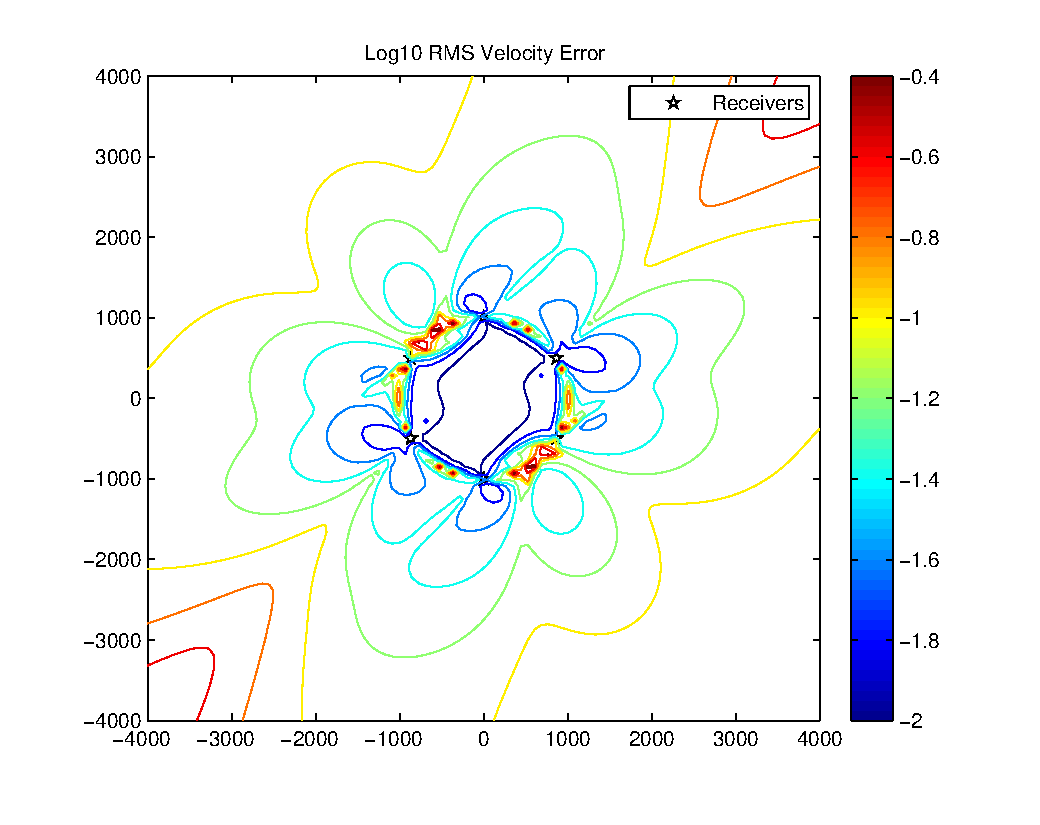
\includegraphics[scale=0.8]{plots-23-Geometry-CRBRandCircularVelocity.eps} 
\end{center}
\caption[Velocity Estimation Preformance Vs. Position for a circular array and a random signal]
{Velocity Estimation Preformance Vs. Position for a circular array and a random signal. We can see that the best performance is achieved inside the circle, where the performance of the algorithm is almost uniform. Outside the circle, the performance decreases as we move away from the center of the circle. It is interesting to notice, that the performance is worst on the line that goes through the center of the circle in the direction of the velocity of the transmitter.}
\label{fig:CRBRandCircularVelocity}
\end{figure}

\subsubsection*{Linear Receivers Array}
For analysing the linear receivers array scenario, we used the receivers array described in figure (\ref{fig:scenario2_geometry}), where there are 6 receivers that are equally spaced on a $2$[km] long line on the $x$-axis.

From figures (\ref{fig:CRBRandLinearPosition}) and (\ref{fig:CRBRandLinearVelocity}) we can learn that for this scenario, the spatial behaviour of the estimation performance of the position and of the estimation performance of the velocity is quite similar.

From both figures, we can learn that the best estimation performance of a linear array is achieved as close as possible to the center of the array. We can see that the farther the transmitter is from the center of the array, the worse the performance.

We notice an interesting phenomenon that occurs on the line on which the receivers lye. On that line, the performance decreases dramatically as we move further away from the receivers array. We can notice this phenomenon both in the position estimation performance and in the velocity estimation performance. This decrease of performance occurs because on that line, the Doppler shift received by all of the receivers is identical, thus, the differential Doppler zeros in all of the receivers, regardless of the velocity of the transmitter or its position on that line. The effect is much more dominant in the velocity estimation, because the velocity estimation depends only on the Doppler shifts, as opposed to the position estimation that also depends on the time delays.

\begin{figure}
\begin{center}
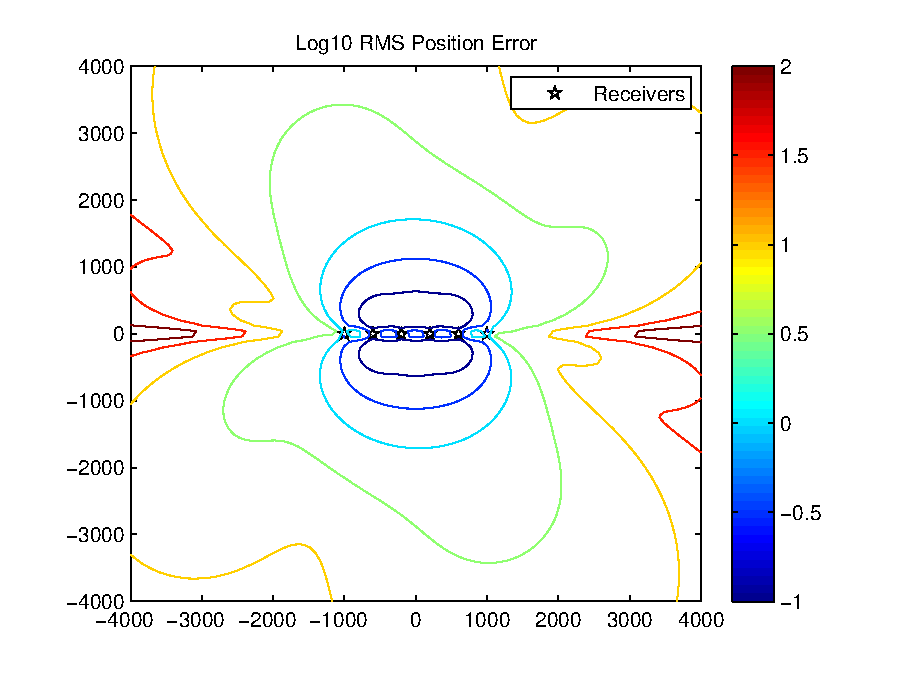
\includegraphics[scale=0.8]{plots-20-Geometry-CRBRandLinearPosition.eps} 
\end{center}
\caption[Position Estimation Preformance Vs. Position for a linear array and a random signal]
{Position Estimation Preformance Vs. Position for a linear array and a random signal}
\label{fig:CRBRandLinearPosition}
\end{figure}

\begin{figure}
\begin{center}
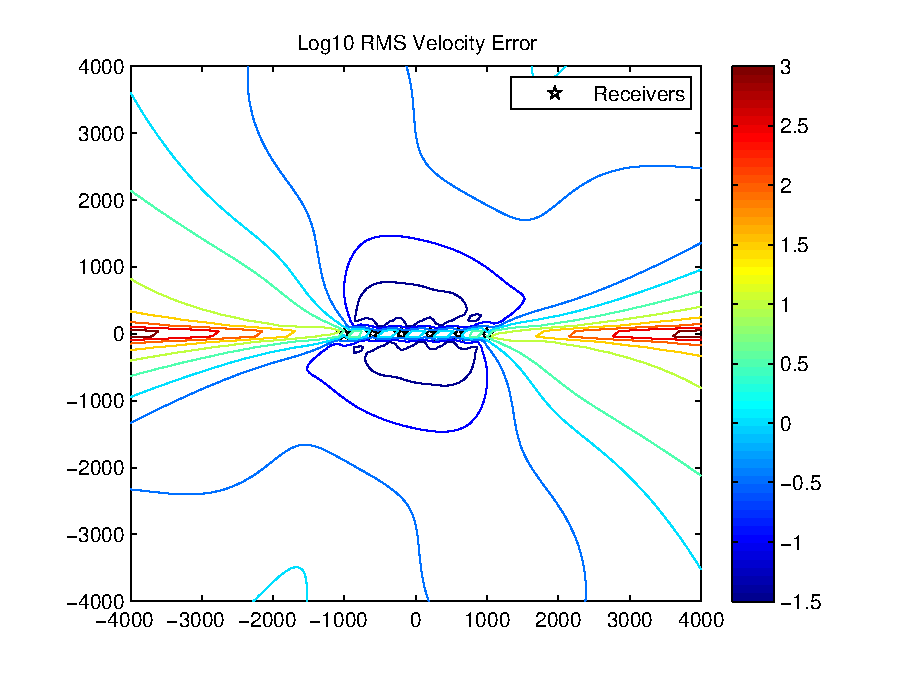
\includegraphics[scale=0.8]{plots-21-Geometry-CRBRandLinearVelocity.eps} 
\end{center}
\caption[Velocity Estimation Preformance Vs. Position for a linear array and a random signal]
{Velocity Estimation Preformance Vs. Position for a linear array and a random signal}
\label{fig:CRBRandLinearVelocity}
\end{figure}

\subsubsection*{Random Receivers Array}
In order to examine a more "realistic" scenario, and in order to see how we can use the intuition acquired in the circular and linear array examples, we examine the performance of a randomly placed receivers array.

In the examined scenario, 6 receivers were placed randomly around the origin. All other scenario parameters, including the velocity of the transmitter are identical to the two previous scenarios.

As can be seen in figure (\ref{fig:CRBRandRandPosition}) and in figure (\ref{fig:CRBRandRandVelocity}) similar behaviour to the previous scenarios is observed.
We can see that the position estimation performance is more isotropic,while the velocity estimation performance is more direction dependent. Similarly to the previous scenarios, we can relate that phenomenon to the fact that the information about the velocity is found only in the Doppler shift of the signals, while the information about the position is found both in the Doppler shifts and in the time delays of the signals.

We can also notice that, similarly to the previous scenarios, the best performance is achieved in the area contained by the receivers. The performance gradually drops as the transmitter is positioned further away from the array of receivers.

\begin{figure}
\begin{center}
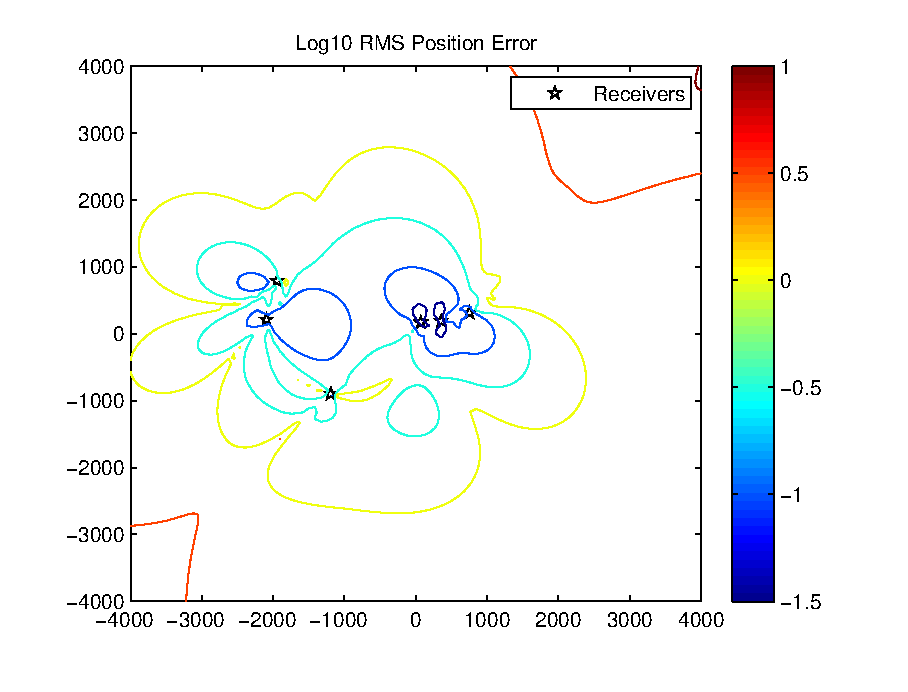
\includegraphics[scale=0.8]{plots-24-Geometry-CRBRandRandPosition.eps} 
\end{center}
\caption[Position Estimation Preformance Vs. Position for a random array and a random signal]
{Position Estimation Preformance Vs. Position for a random array and a random signal}
\label{fig:CRBRandRandPosition}
\end{figure}




\begin{figure}
\begin{center}
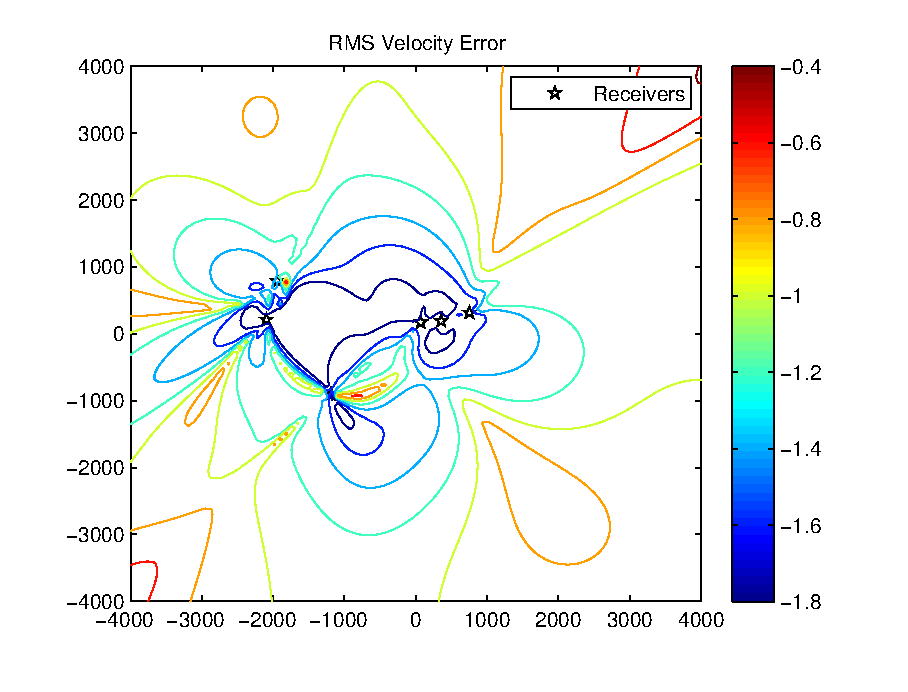
\includegraphics[scale=0.8]{plots-25-Geometry-CRBRandRandVelocity.eps} 
\end{center}
\caption[Velocity Estimation Preformance Vs. Position for a random array and a random signal]
{Velocity Estimation Preformance Vs. Position for a random array and a random signal}
\label{fig:CRBRandRandVelocity}
\end{figure}

%\subsection{Performance vs. Antenna Elements - Circular Array}
%\subsection{Performance vs. Antenna Elements - Linear Array}
%\subsection{Performance vs. Bandwidth}
%\subsection{Performance vs. Transmitter Distance}
%\subsection{Performance vs. Transmitter velocity}
%\subsection{Performance vs. Observation Time}
%\section{Dynamic Scenario}
%\subsection{Performance vs. Number of Observations}
